\documentclass[11pt,oneside]{article}
\usepackage[T1]{fontenc}
\usepackage[utf8]{inputenc}
% \usepackage{lmodern}
%\usepackage[adobe-utopia,uppercase=upright,greeklowercase=upright]{mathdesign}
\usepackage[adobe-utopia]{mathdesign}
%\usepackage{minionpro}
% \usepackage{pifont}
% \usepackage{amssymb}
\usepackage{amsmath}
\usepackage[francais]{babel}
% \usepackage[francais]{varioref}
\usepackage[dvips]{graphicx}

\usepackage{framed}
\usepackage[normalem]{ulem}
\usepackage{fancyhdr}
\usepackage{titlesec}
\usepackage{vmargin}
\usepackage{longtable}

\usepackage{ifthen}


%\usepackage{epsfig}
\usepackage{subfig}

\usepackage{multirow}
\usepackage{multicol} % Portions de texte en colonnes
\usepackage{flafter}%floatants après la référence



\usepackage{color}
\usepackage{colortbl}


\definecolor{gris25}{gray}{0.75}
\definecolor{bleu}{RGB}{18,33,98}
\definecolor{bleuf}{RGB}{42,94,171}
\definecolor{bleuc}{RGB}{231,239,247}
\definecolor{rougef}{RGB}{185,18,27}
\definecolor{rougec}{RGB}{255,230,231}
\definecolor{vertf}{RGB}{103,126,82}
\definecolor{vertc}{RGB}{220,255,191}

\newenvironment{rem}[1][\hsize]%
{%
    \def\FrameCommand
    {%
\rotatebox{90}{\textit{\textsf{Remarque}}} 
        {\color{bleuf}\vrule width 3pt}%
        \hspace{0pt}%must no space.
        \fboxsep=\FrameSep\colorbox{bleuc}%
    }%
    \MakeFramed{\hsize#1\advance\hsize-\width\FrameRestore}%
}%
{\endMakeFramed}%


\newenvironment{savoir}[1][\hsize]%
{%
    \def\FrameCommand
    {%
\rotatebox{90}{\textit{\textsf{Savoir}}} 
        {\color{bleuf}\vrule width 3pt}%
        \hspace{0pt}%must no space.
        \fboxsep=\FrameSep\colorbox{bleuc}%
    }%
    \MakeFramed{\hsize#1\advance\hsize-\width\FrameRestore}%
}%
{\endMakeFramed}%

\newenvironment{prob}[1][\hsize]%
{%
    \def\FrameCommand%
    {%
\rotatebox{90}{\textit{\textsf{ Problématique}}} 
        {\color{rougef}\vrule width 3pt}%
        \hspace{0pt}%must no space.
        \fboxsep=\FrameSep\colorbox{rougec}%
    }%
    \MakeFramed{\hsize#1\advance\hsize-\width\FrameRestore}%
}%
{\endMakeFramed}%

\newenvironment{obj}[1][\hsize]%
{%
    \def\FrameCommand%
    {%
\rotatebox{90}{\textit{\textsf{ $\;$}}} 
        {\color{rougef}\vrule width 3pt}%
        \hspace{0pt}%must no space.
        \fboxsep=\FrameSep\colorbox{rougec}%
    }%
    \MakeFramed{\hsize#1\advance\hsize-\width\FrameRestore}%
}%
{\endMakeFramed}%

\newenvironment{defi}[1][\hsize]%
{%
    \def\FrameCommand%
    {%
\rotatebox{90}{\textit{\textsf{Définition\\}}} 
        {\color{bleuf}\vrule width 3pt}%
        \hspace{0pt}%must no space.
        \fboxsep=\FrameSep\colorbox{bleuc}%
    }%
    \MakeFramed{\hsize#1\advance\hsize-\width\FrameRestore}%
}%
{\endMakeFramed}%


\newenvironment{hypo}[1][\hsize]%
{%
    \def\FrameCommand%
    {%
\rotatebox{90}{\textit{\textsf{Hypothèse\\}}} 
        {\color{bleuf}\vrule width 3pt}%
        \hspace{0pt}%must no space.
        \fboxsep=\FrameSep\colorbox{bleuc}%
    }%
    \MakeFramed{\hsize#1\advance\hsize-\width\FrameRestore}%
}%
{\endMakeFramed}%


\newenvironment{prop}[1][\hsize]%
{%
    \def\FrameCommand%
    {%
\rotatebox{90}{\textit{\textsf{Propriété\\}}} 
        {\color{bleuf}\vrule width 3pt}%
        \hspace{0pt}%must no space.
        \fboxsep=\FrameSep\colorbox{bleuc}%
    }%
    \MakeFramed{\hsize#1\advance\hsize-\width\FrameRestore}%
}%
{\endMakeFramed}%

\newenvironment{props}[1][\hsize]%
{%
    \def\FrameCommand%
    {%
\rotatebox{90}{\textit{\textsf{Propriétés\\}}} 
        {\color{bleuf}\vrule width 3pt}%
        \hspace{0pt}%must no space.
        \fboxsep=\FrameSep\colorbox{bleuc}%
    }%
    \MakeFramed{\hsize#1\advance\hsize-\width\FrameRestore}%
}%
{\endMakeFramed}%

\newenvironment{exemple}[1][\hsize]%
{%
    \def\FrameCommand%
    {%
\rotatebox{90}{\textit{\textsf{Exemple\\}}} 
        {\color{vertf}\vrule width 3pt}%
        \hspace{0pt}%must no space.
        \fboxsep=\FrameSep\colorbox{vertc}%
    }%
    \MakeFramed{\hsize#1\advance\hsize-\width\FrameRestore}%
}%
{\endMakeFramed}%

\newenvironment{resultat}[1][\hsize]%
{%
    \def\FrameCommand%
    {%
\rotatebox{90}{\textit{\textsf{Résultat\\}}} 
        {\color{rougef}\vrule width 3pt}%
        \hspace{0pt}%must no space.
        \fboxsep=\FrameSep\colorbox{rougec}%
    }%
    \MakeFramed{\hsize#1\advance\hsize-\width\FrameRestore}%
}%
{\endMakeFramed}%

\newenvironment{methode}[1][\hsize]%
{%
    \def\FrameCommand%
    {%
\rotatebox{90}{\textit{\textsf{Méthode\\}}} 
        {\color{rougef}\vrule width 3pt}%
        \hspace{0pt}%must no space.
        \fboxsep=\FrameSep\colorbox{rougec}%
    }%
    \MakeFramed{\hsize#1\advance\hsize-\width\FrameRestore}%
}%
{\endMakeFramed}%

\newenvironment{theo}[1][\hsize]%
{%
    \def\FrameCommand%
    {%
\rotatebox{90}{\textit{\textsf{Théorème\\}}} 
        {\color{rougef}\vrule width 3pt}%
        \hspace{0pt}%must no space.
        \fboxsep=\FrameSep\colorbox{rougec}%
    }%
    \MakeFramed{\hsize#1\advance\hsize-\width\FrameRestore}%
}%
{\endMakeFramed}%

\newenvironment{warn}[1][\hsize]%
{%
    \def\FrameCommand%
    {%
\rotatebox{90}{\textit{\textsf{Attention\\}}} 
        {\color{rougef}\vrule width 3pt}%
        \hspace{0pt}%must no space.
        \fboxsep=\FrameSep\colorbox{rougec}%
    }%
    \MakeFramed{\hsize#1\advance\hsize-\width\FrameRestore}%
}%
{\endMakeFramed}%

% \usepackage{pstricks}
%\usepackage{minitoc}
% \setcounter{minitocdepth}{4}

\setcounter{tocdepth}{2}

% \mtcselectlanguage{french} 

%\usepackage{draftcopy}% "Brouillon"
% \usepackage{floatflt}
\usepackage{psfrag}
%\usepackage{listings} % Permet d'insérer du code de programmation
\renewcommand{\baselinestretch}{1.2}

% Changer la numérotation des figures :
% ------------------------------------
% \makeatletter
% \renewcommand{\thefigure}{\ifnum \c@section>\z@ \thesection.\fi
%  \@arabic\c@figure}
% \@addtoreset{figure}{section}
% \makeatother
 


%%%%%%%%%%%%
% Définition des vecteurs %
%%%%%%%%%%%%
 \newcommand{\vect}[1]{\overrightarrow{#1}}

%%%%%%%%%%%%
% Définition des torseusr %
%%%%%%%%%%%%

 \newcommand{\torseur}[1]{%
\left\{{#1}\right\}
}

\newcommand{\torseurcin}[3]{%
\left\{\mathcal{#1} \left(#2/#3 \right) \right\}
}

\newcommand{\torseurstat}[3]{%
\left\{\mathcal{#1} \left(#2\rightarrow #3 \right) \right\}
}

 \newcommand{\torseurc}[8]{%
%\left\{#1 \right\}=
\left\{
{#1}
\right\}
 = 
\left\{%
\begin{array}{cc}%
{#2} & {#5}\\%
{#3} & {#6}\\%
{#4} & {#7}\\%
\end{array}%
\right\}_{#8}%
}

 \newcommand{\torseurcol}[7]{
\left\{%
\begin{array}{cc}%
{#1} & {#4}\\%
{#2} & {#5}\\%
{#3} & {#6}\\%
\end{array}%
\right\}_{#7}%
}

 \newcommand{\torseurl}[3]{%
%\left\{\mathcal{#1}\right\}_{#2}=%
\left\{%
\begin{array}{l}%
{#1} \\%
{#2} %
\end{array}%
\right\}_{#3}%
}

 \newcommand{\vectv}[3]{%
\vect{V\left( {#1} \in {#2}/{#3}\right)}
}


\newcommand{\vectf}[2]{%
\vect{R\left( {#1} \rightarrow {#2}\right)}
}

\newcommand{\vectm}[3]{%
\vect{\mathcal{M}\left( {#1}, {#2} \rightarrow {#3}\right)}
}


 \newcommand{\vectg}[3]{%
\vect{\Gamma \left( {#1} \in {#2}/{#3}\right)}
}

 \newcommand{\vecto}[2]{%
\vect{\Omega\left( {#1}/{#2}\right)}
}
% }$$\left\{\mathcal{#1} \right\}_{#2} =%
% \left\{%
% \begin{array}{c}%
%  #3 \\%
%  #4 %
% \end{array}%
% \right\}_{#5}}

%  ------------------------------------------
% | Modification du formatage des sections : | 
%  ------------------------------------------

% Grands titres :
% ---------------

\newcommand{\titre}[1]{%
\begin{center}
      \bigskip
      \rule{\textwidth}{1pt}
      \par\vspace{0.1cm}
      
      \textbf{\large #1}
      \par\rule{\textwidth}{1pt}
    \end{center}
    \bigskip
  }

% Supprime le numéro du chapitre dans la numérotation des sections:
% -----------------------------------------------------------------
\makeatletter
\renewcommand{\thesection}{\@arabic\c@section}
\makeatother


% \titleformat{\chapter}[display]
% {\normalfont\Large\filcenter}
% {}
% {1pc}
% {\titlerule[1pt]
%   \vspace{1pc}%
%   \Huge}[\vspace{1ex}%
% \titlerule]


%%%% Chapitres Comme PY Pechard %%%%%%%%%
% numéro du chapitre
\DeclareFixedFont{\chapnumfont}{OT1}{phv}{b}{n}{80pt}
% pour le mot « Chapitre »
\DeclareFixedFont{\chapchapfont}{OT1}{phv}{m}{it}{40pt}
% pour le titre
\DeclareFixedFont{\chaptitfont}{T1}{phv}{b}{n}{25pt}

\definecolor{gris}{gray}{0.75}
\titleformat{\chapter}[display]%
	{\sffamily}%
	{\filleft\chapchapfont\color{gris}\chaptertitlename\
	\\
	\vspace{12pt}
	\chapnumfont\thechapter}%
	{16pt}%
	{\filleft\chaptitfont}%
	[\vspace{6pt}\titlerule\titlerule\titlerule]

%%%%  Fin Chapitres Comme PY Pechard %%%%%%%%%


% Section, subsection, subsubsection sans serifs :
% % ----------------------------------------------

% \makeatletter
% \renewcommand{\section}{\@startsection{section}{0}{0mm}%
% {\baselineskip}{.3\baselineskip}%
% {\normalfont\sffamily\Large\textbf}}%
% \makeatother

\makeatletter
\renewcommand{\@seccntformat}[1]{{\textcolor{bleu}{\csname
the#1\endcsname}\hspace{0.5em}}}
\makeatother

\makeatletter
\renewcommand{\section}{\@startsection{section}{1}{\z@}%
                       {-4ex \@plus -1ex \@minus -.4ex}%
                       {1ex \@plus.2ex }%
                       {\normalfont\Large\sffamily\bfseries}}%
\makeatother
 
\makeatletter
\renewcommand{\subsection}{\@startsection {subsection}{2}{\z@}
                          {-3ex \@plus -0.1ex \@minus -.4ex}%
                          {0.5ex \@plus.2ex }%
                          {\normalfont\large\sffamily\bfseries}}
\makeatother
 
\makeatletter
\renewcommand{\subsubsection}{\@startsection {subsubsection}{3}{\z@}
                          {-2ex \@plus -0.1ex \@minus -.2ex}%
                          {0.2ex \@plus.2ex }%
                          {\normalfont\large\sffamily\bfseries}}
\makeatother
 
\makeatletter             
\renewcommand{\paragraph}{\@startsection{paragraph}{4}{\z@}%
                                    {-2ex \@plus-.2ex \@minus .2ex}%
                                    {0.1ex}%               
{\normalfont\sffamily\bfseries}}
\makeatother
 
\makeatletter
\renewcommand{\subparagraph}{\@startsection{subparagraph}{5}{\z@}%
                                       {-2ex \@plus-.1ex \@minus .2ex}%
                                       {0.1ex}%
				    {\normalfont\normalsize\sffamily\bfseries}}
\makeatletter
% \makeatletter
% \renewcommand{\subsection}{\@startsection{subsection}{1}{2mm}%
% {\baselineskip}{.3\baselineskip}%
% {\normalfont\sffamily\large\textbf}}%
% \makeatother
% 
% \makeatletter
% \renewcommand{\subsubsection}{\@startsection{subsubsection}{2}{4mm}%
% {\baselineskip}{.15\baselineskip}%
% {\normalfont\sffamily\large\textbf}}%
% \makeatother
% 
% \makeatletter
% \renewcommand{\paragraph}{\@startsection{paragraph}{3}{6mm}%
% {\baselineskip}{.15\baselineskip}%
% {\normalfont\sffamily\large\textbf}}%
% \makeatother
 
\setcounter{secnumdepth}{4}


%  --------
% | Marges |
%  --------


% \setmarginsrb{2.5cm}{1.5cm}{2.5cm}{2cm}{1cm}{1cm}{1cm}{1cm}
\setmarginsrb{1.5cm}{1cm}{1cm}{1.5cm}{1cm}{1cm}{1cm}{1cm}

% Changer les marges localement :
% -----------------------------
\newenvironment{changemargin}[2]{\begin{list}{}{%
\setlength{\topsep}{0pt}%
\setlength{\leftmargin}{0pt}%
\setlength{\rightmargin}{0pt}%
\setlength{\listparindent}{\parindent}%
\setlength{\itemindent}{\parindent}%
\setlength{\parsep}{0pt plus 1pt}%
\addtolength{\leftmargin}{#1}%
\addtolength{\rightmargin}{#2}%
}\item }{\end{list}}



\usepackage{pst-solides3d}
\usepackage{titletoc}
\titlecontents{chapter}[+3pc]
  {\addvspace{10pt}\sffamily\bfseries}
{\contentslabel[{\pscirclebox[fillstyle=solid,fillcolor=gray!25,
linecolor=gray!25,framesep=4pt]{\textcolor{white}{\thecontentslabel}}}]{2.5pc}}
  {}
  {\dotfill \normalfont\thecontentspage\ }

\titlecontents{section}[3pc]
  {\addvspace{2pt}\sffamily}
  {\contentslabel[\thecontentslabel]{1.8pc}}
  {}
  {\dotfill \normalfont\thecontentspage\ }

\titlecontents{subsection}[5pc]
  {\addvspace{2pt}\sffamily}
  {\contentslabel[\thecontentslabel]{1.8pc}}
  {}
  {\dotfill \normalfont\thecontentspage\ }

\titlecontents{subsubsection}[8pc]
  {\addvspace{2pt}\sffamily}
  {\contentslabel[\thecontentslabel]{3pc}}
  {}
  {\dotfill \normalfont\thecontentspage\ }
%{\;\titlerule\;\normalfont\thecontentspage\ }

\titlecontents{paragraph}[9pc]
  {\addvspace{2pt}\sffamily}
  {\contentslabel[\thecontentslabel]{3.5pc}}
  {}
  {\dotfill \normalfont\thecontentspage\ }



\usepackage[raccourcis]{FAST}
\usepackage[%
    pdftitle={Produits Procédés Matériaux -- },
    pdfauthor={Xavier Pessoles},
    colorlinks=true,
    linkcolor=blue,
    citecolor=magenta]{hyperref}

\usepackage{pifont}


% \makeatletter \let\ps@plain\ps@empty \makeatother
%% DEBUT DU DOCUMENT
%% =================
\sloppy
\hyphenpenalty 10000

\newcommand{\Pointilles}[1][3]{%
\multido{}{#1}{\makebox[\linewidth]{\dotfill}\\[\parskip]
}}


\colorlet{shadecolor}{orange!15}

\newtheorem{theorem}{Theorem}


\begin{document}


\newboolean{prof}
\setboolean{prof}{true}
%------------- En tetes et Pieds de Pages ------------
\pagestyle{fancy}
\renewcommand{\headrulewidth}{0pt}

\fancyhead{}
\fancyhead[L]{%
\noindent\noindent\begin{minipage}[c]{2.6cm}
%Lycée Rouvière PTSI

\includegraphics[width=2cm]{png/logo_ptsi.png}%
\end{minipage}
}


\fancyhead[C]{\rule{12cm}{.5pt}}

\fancyhead[R]{%
\noindent\begin{minipage}[c]{3cm}
\begin{flushright}
\footnotesize{\textit{\textsf{Sciences Industrielles\\ de l'Ingénieur}}}%
\end{flushright}
\end{minipage}
}

\renewcommand{\footrulewidth}{0.2pt}

\fancyfoot[C]{\footnotesize{\bfseries \thepage}}
\fancyfoot[L]{\footnotesize{2012 -- 2013} \\ X. \textsc{Pessoles}}
\ifthenelse{\boolean{prof}}{%
\fancyfoot[R]{\footnotesize{Cours -- CI 6 : PPM -- P}}
}{%
\fancyfoot[R]{\footnotesize{Cours -- CI 6 : PPM}}
}



\begin{center}
 \huge\textsc{CI 6 -- PPM -- Produits Procédés Matériaux}

 \large\textsc{Élaboration des pièces mécaniques. Introduction de la chaîne numérique.}
\end{center}

\begin{center}
 \LARGE\textsc{Chapitre 10 -- Usinage -- Fraisage}
\end{center}

%\begin{flushright}
%\textit{D'après documents de Jean-Pierre Pupier}
%\end{flushright}

\vspace{.5cm}


\begin{minipage}[c]{.23\linewidth}
\begin{center}
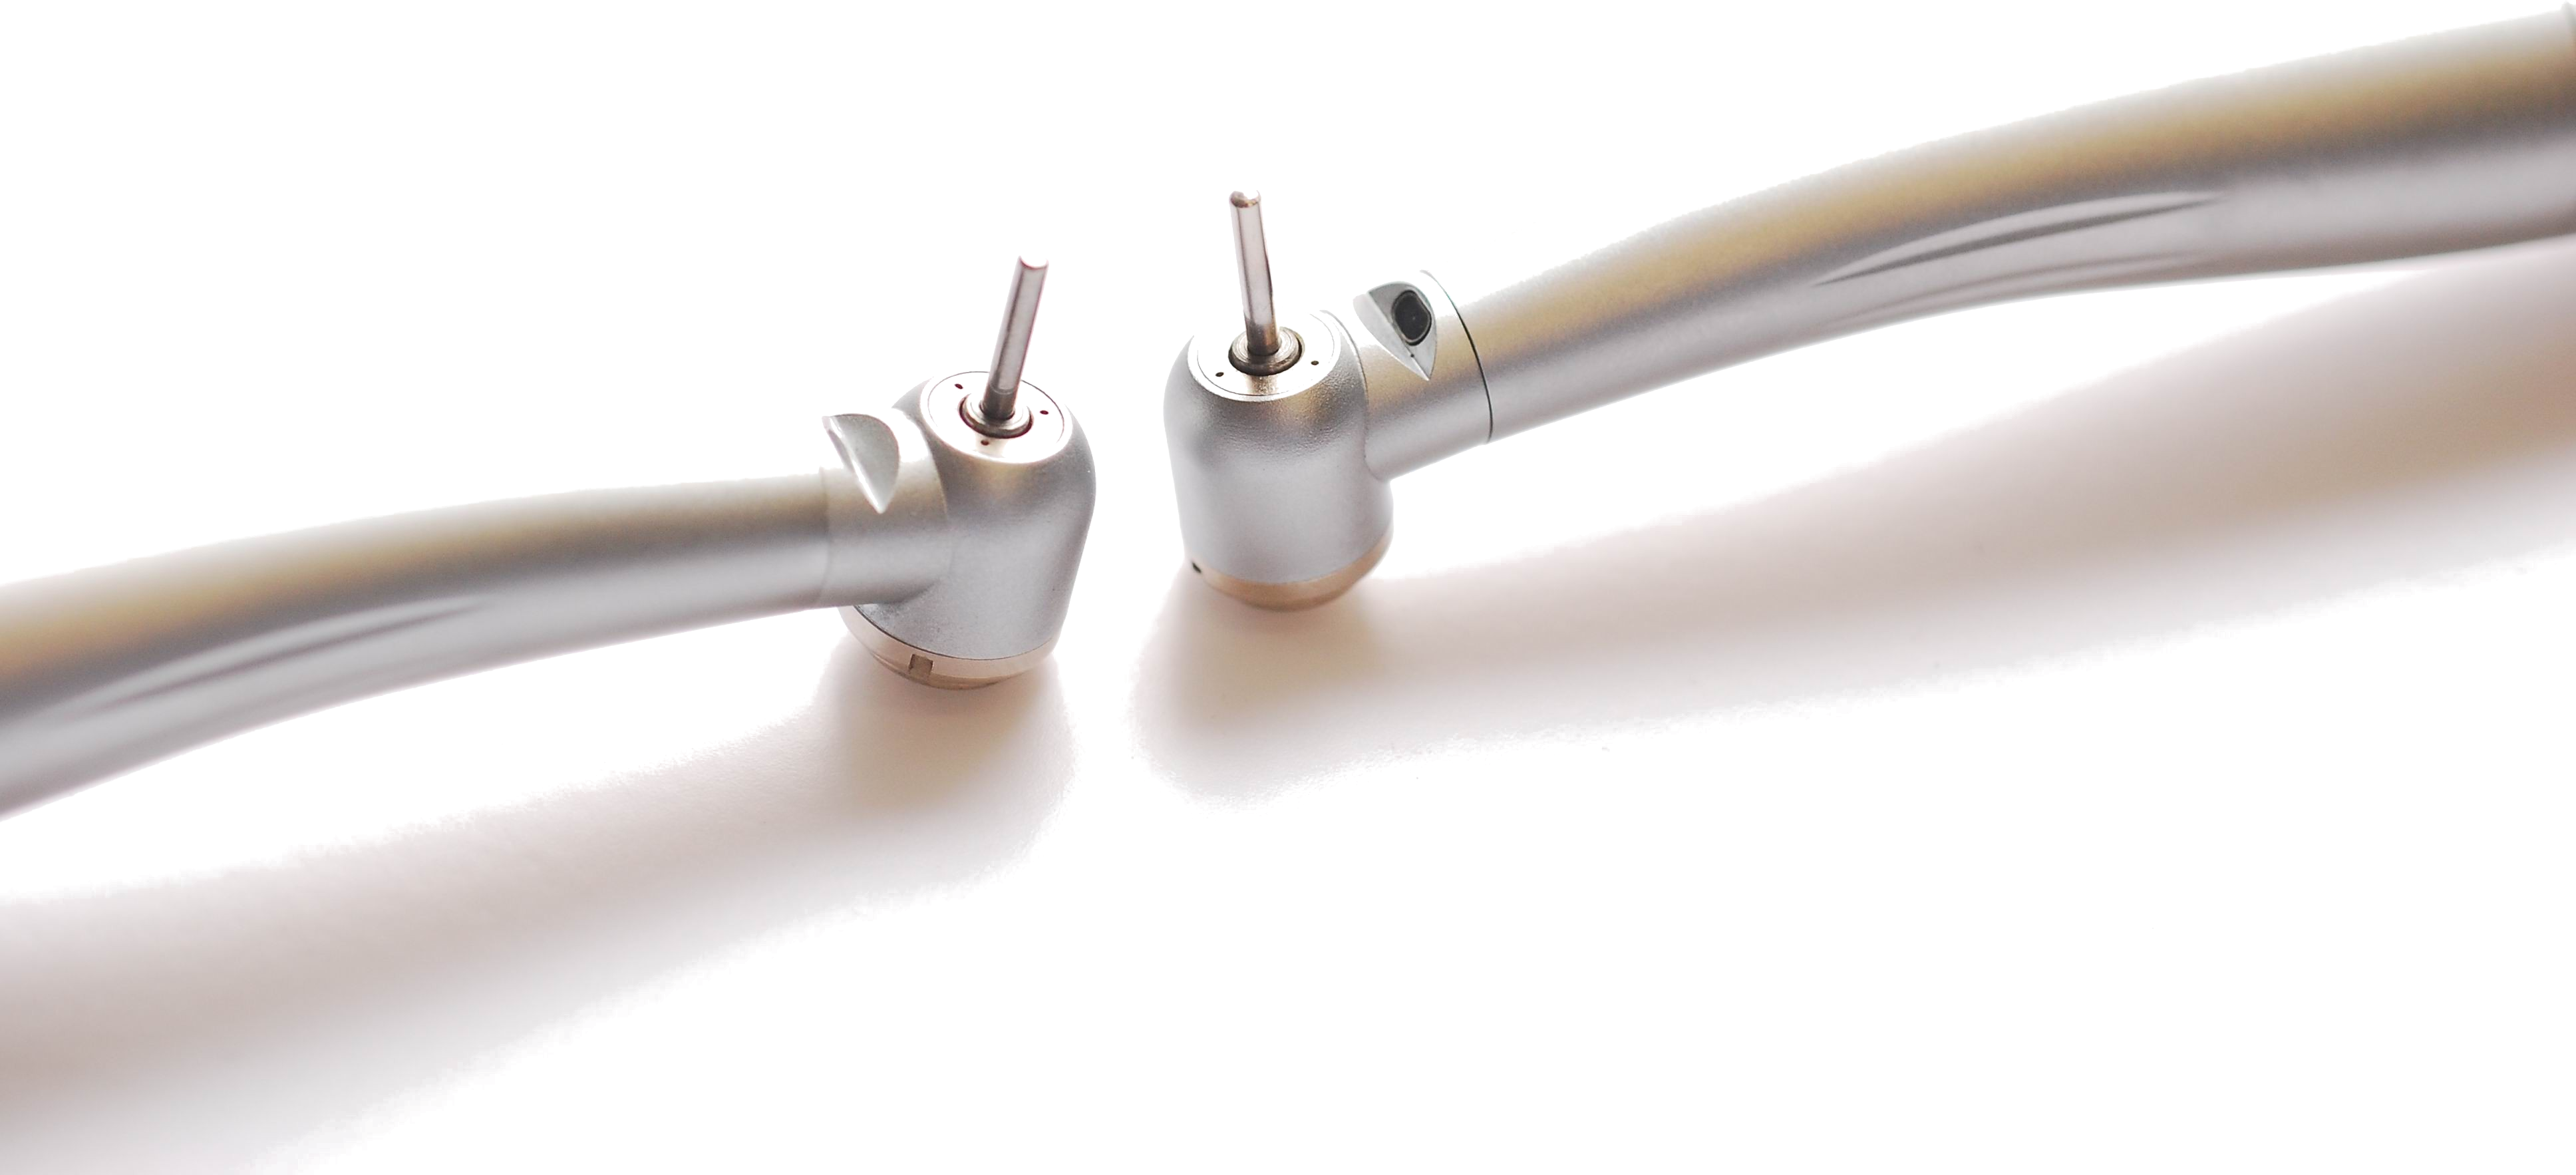
\includegraphics[height=2cm]{png/fraise_dentiste}

\textit{Fraise de dentiste \cite{dent}}
\end{center}
\end{minipage} \hfill
\begin{minipage}[c]{.23\linewidth}
\begin{center}
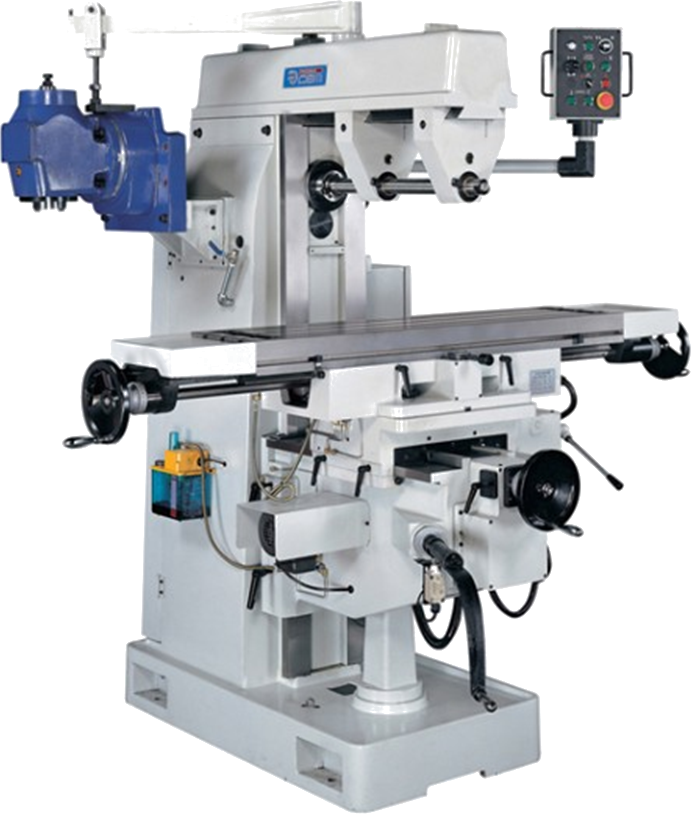
\includegraphics[height=2.5cm]{png/fraise_conventionnelle}

\textit{Fraise conventionnelle \cite{conventionnel}}
\end{center}
\end{minipage} \hfill
\begin{minipage}[c]{.23\linewidth}
\begin{center}
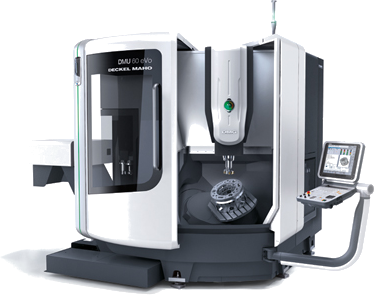
\includegraphics[height=2.5cm]{png/5axes}

\textit{Centre d'usinage 5 axes \cite{5axes}}
\end{center}
\end{minipage}\hfill
\begin{minipage}[c]{.23\linewidth}
\begin{center}
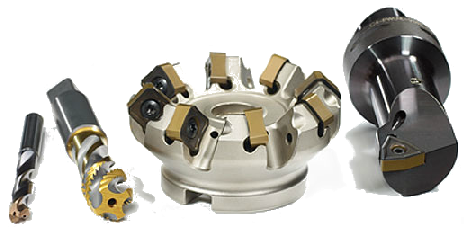
\includegraphics[height=2cm]{png/fraises}

\textit{Outils de fraisage \cite{fraises}}
\end{center}
\end{minipage}

\vspace{.5cm}


\begin{center}
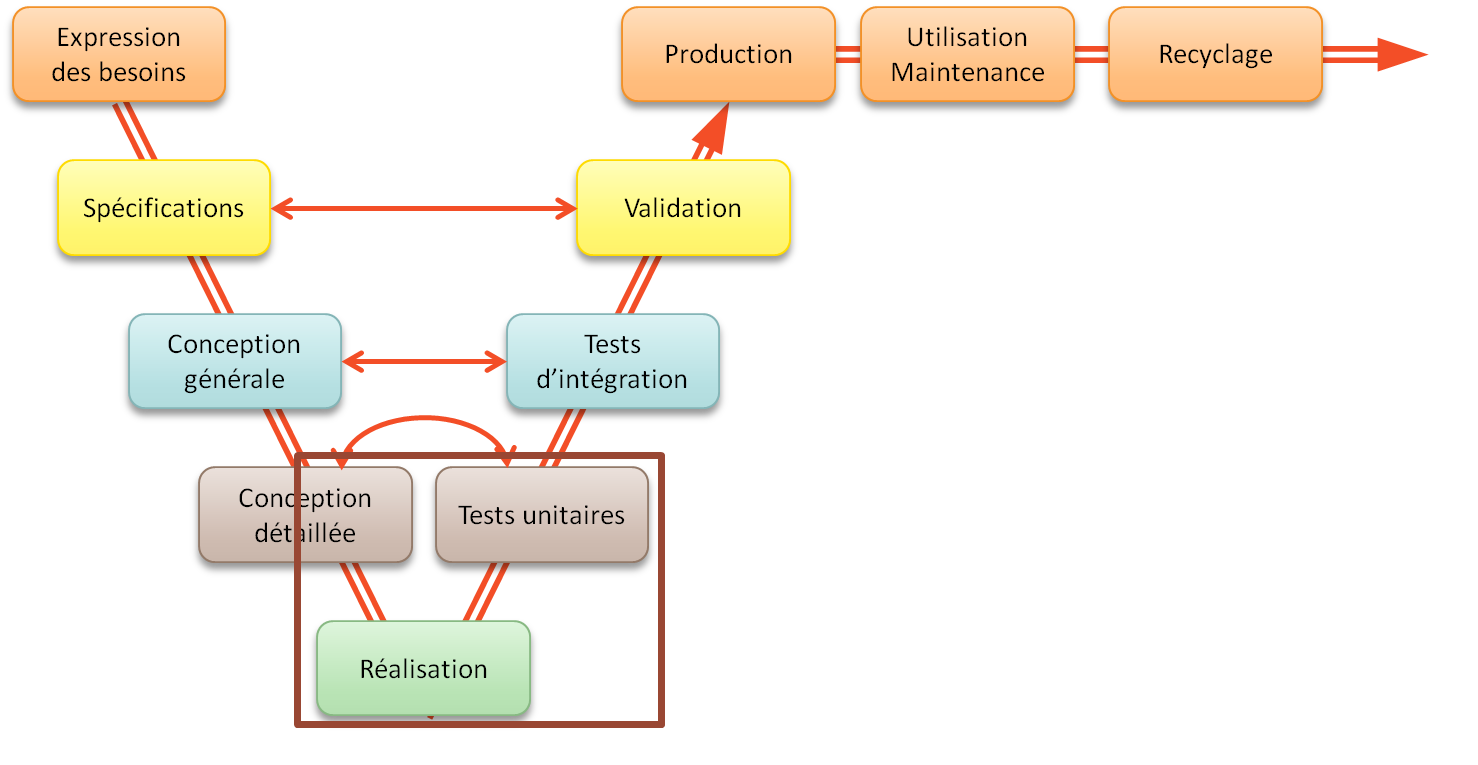
\includegraphics[height=7cm]{png/cycleV}
\end{center}

%\begin{center}
%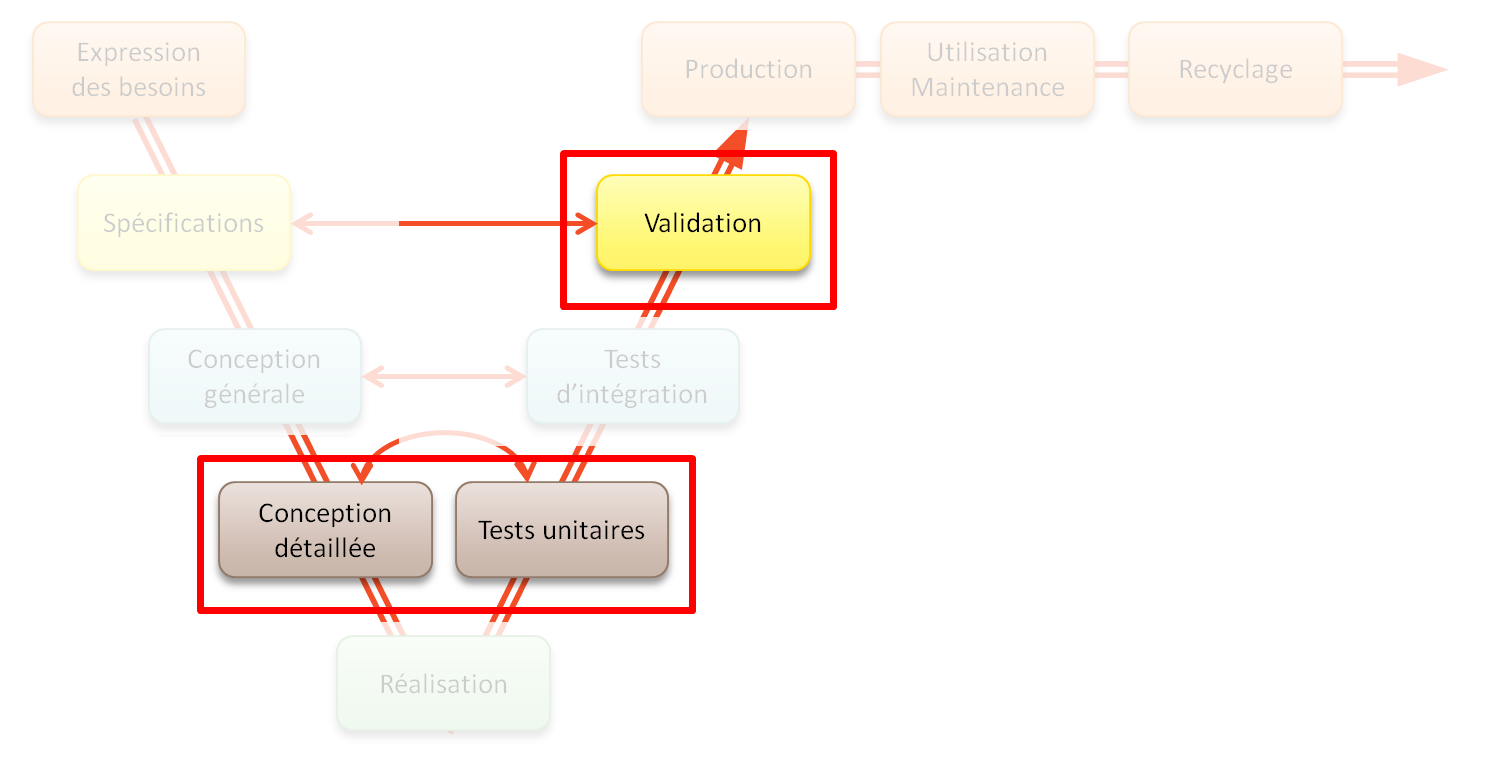
\includegraphics[width=.9\textwidth]{png/cyclev.png}

%\textit{Cycle de conception d'un produit}
%\end{center}

%\begin{prob}
%\textsc{Problématique :}
%\begin{itemize}
%\item %Quelles sont les conditions fonctionnelles permettant le fonctionnement du système ?
%\item %Quelle est la chaîne de côte unidirectionnelle correspondant à une condition donnée ?
%\end{itemize}
%\end{prob}



\begin{savoir}
\textsc{Savoirs :}
\begin{itemize}
\item Présenter de façon structurée un usinage en fraisage :
\begin{itemize}
\item Les éléments de la cellule élémentaire d'usinage
\item Les opérations de fraisage
\end{itemize}
\end{itemize}
\end{savoir}
 

\setlength{\parskip}{0ex plus 0.2ex minus 0ex}
 \renewcommand{\contentsname}{}
 \renewcommand{\baselinestretch}{1}

\tableofcontents

 \renewcommand{\baselinestretch}{1.2}
\setlength{\parskip}{2ex plus 0.5ex minus 0.2ex}

% \vspace{1cm}
\textit{Ce document évolue. Merci de signaler toutes erreurs ou coquilles.}

\section{Présentation}

\subsection{Définition}

\begin{defi}
\textbf{Fraisage}

\begin{minipage}[c]{.55\linewidth}
Le fraisage est une opération d'usinage qui permet de réaliser tout type de surface. Le \textbf{mouvement de coupe} est assuré par une rotation de l'outil. Le \textbf{mouvement d'avance} est assuré par des translations. Suivant la structure de la machine, les translations peuvent être réalisées par la pièce ou par l'outil. 
\end{minipage}\hfill
\begin{minipage}[c]{.4\linewidth}
\begin{center}
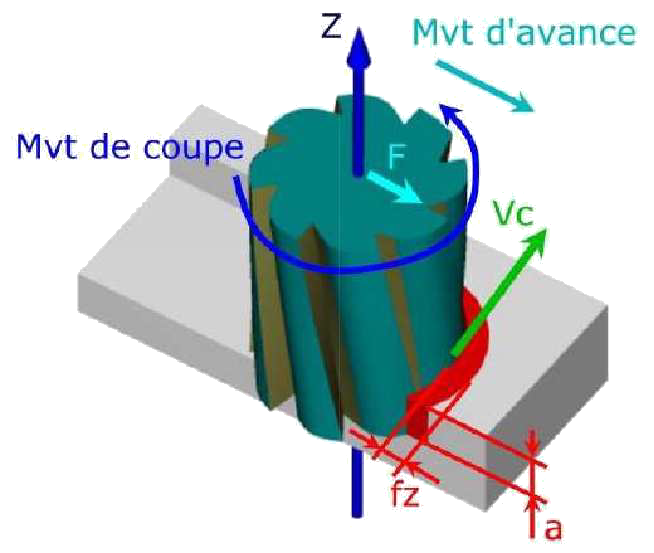
\includegraphics[width=.95\textwidth]{png/mvt_fraisage}
\end{center}
\end{minipage}
\end{defi}


\subsection{Cellule élémentaire d'usinage}

\begin{minipage}[c]{.55\linewidth}
Les systèmes de production sont constitués des éléments suivants : 
\begin{itemize}
\item la machine : dans notre cas la machine est une fraiseuse. Elle est dite conventionnel lorsque les déplacements des axes sont directement générés par un opérateur. Il est dit à commande numérique lorsque les déplacements des axes et la gestion de la machine se fait par une commande numérique, autrement dit, un ordinateur;
\item le porte-outil permet de faire l'interface entre la broche de la machine et l'outil; 
\item l'outil coupant permet de réaliser des opérations de fraisage sur une pièce;
\item le porte pièce permet de faire l'interface entre la machine et la pièce;
\item la pièce est le produit à usiner. 
\end{itemize}
\end{minipage}\hfill
\begin{minipage}[c]{.4\linewidth}
\begin{center}
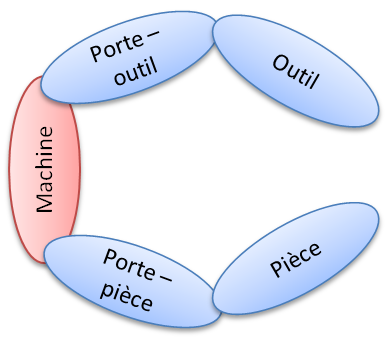
\includegraphics[width=.95\textwidth]{png/ceu}
\end{center}
\end{minipage}
\section{Les machines}
\subsection{Axes normalisés}
Sur les centres d'usinage, le choix des axes de déplacement est normalisé. Cela est notamment nécessaire dans le cas de la programmation des commandes numériques afin qu'un programme soit plus facilement transmissible d'une machine à une autre. 

Le nombre d'axes est donné par les mouvements d'avance. Le plus communément les fraiseuses sont des machines à \textbf{3 axes}.

D'après la norme :
\begin{itemize}
\item l'axe $\vect{Z_m}$ est parallèle à l'axe de rotation de la broche. Le sens positif est donné par l'éloignement de l'outil par rapport à la pièce;
\item l'axe $\vect{X_m}$ est perpendiculaire à l'axe $\vect{Z_m}$. Il a la direction du plus grand déplacement. Le sens positif est donné par l'éloignement de l'outil par rapport à la pièce;
\item l'axe $\vect{Y_m}$ est tel que le trièdre $(\vect{X_m},\vect{Y_m},\vect{Z_m})$ soit orthonormé direct. 
\end{itemize}


\begin{center}
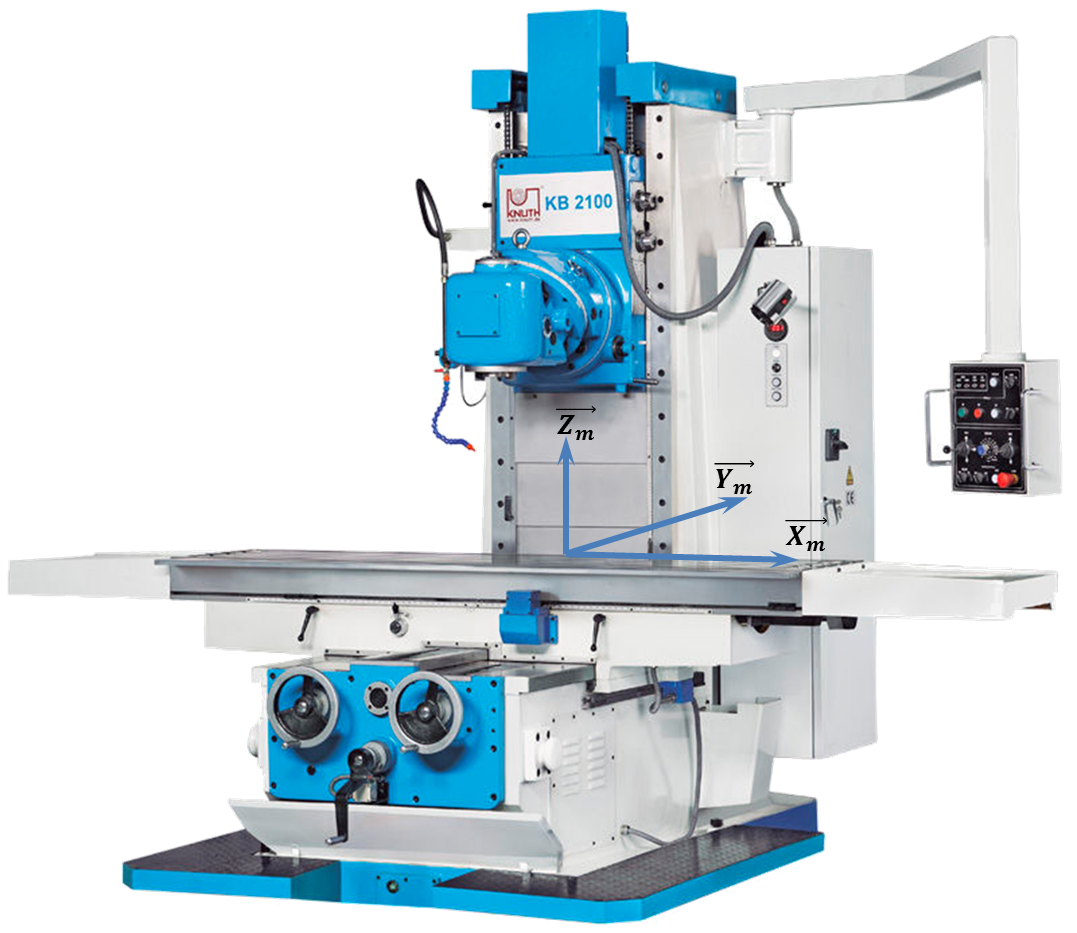
\includegraphics[height=7cm]{png/axes_normalises}

\textit{Axes normalisés sur une fraiseuse conventionnelle}
\end{center}


On rencontre aussi couramment des centres d'usinage 4 et 5 axes. Dans ces cas, les quatrièmes et cinquièmes axes sont des aces de rotation. Si l'axe de rotation est parallèle à l'axe $\vect{X_m}$, il est noté $A_m$, l'axe de rotation parallèle à $\vect{Y_m}$ est noté $B_m$, l'axe de rotation parallèle à $\vect{Z_m}$ est noté $C_m$.

\begin{center}
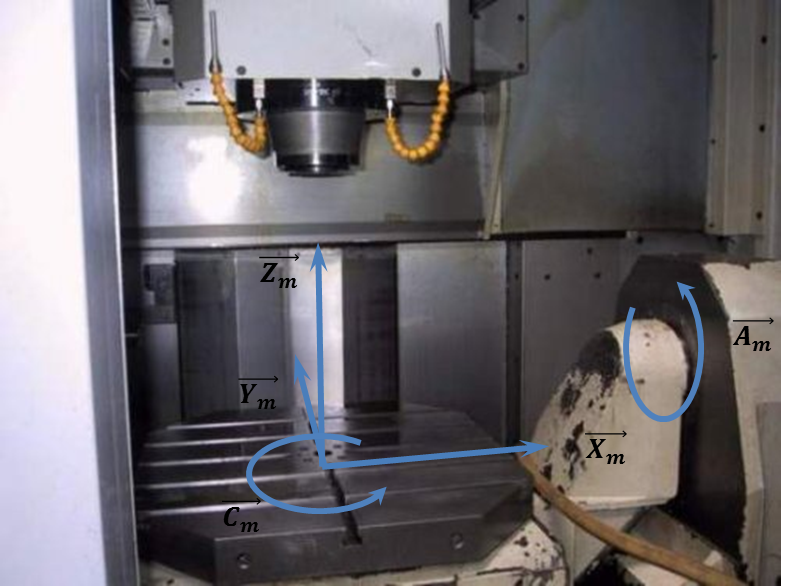
\includegraphics[height=6cm]{png/axes_normalises_2}

\textit{Axes normalisés sur un centre d'usinage 5 axes}
\end{center}

\subsection{Les machines conventionnelles}
Sur les machines conventionnelles, une fois la vitesse d'avance fixée, les distances de déplacement sont directement gérées par l'opérateur. 

Les mouvements des machines conventionnelles sont assurés par un moteur asynchrone. Elles sont équipées de deux  boîtes de vitesses mécaniques. La première permet de fixer la vitesse d'avance de l'outil. La seconde permet de choisir la fréquence de rotation de la broche. 

%\begin{center}
%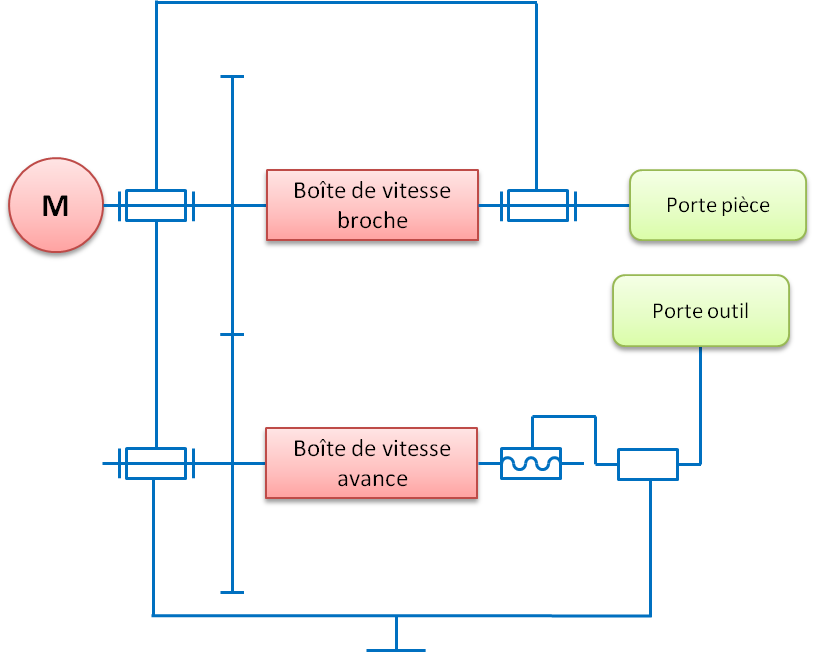
\includegraphics[width=.7\textwidth]{png/schema_tour_conv}
%\end{center}


\subsection{Les machines à commandes numériques}
Les machines à commandes numériques sont équipées d'un moteur asynchrone pour la broche ainsi que d'un variateur de vitesse permettant un choix de vitesse plus précis qu'avec une boîte de vitesse. Des moteurs à courants continus permettent le déplacement sur les axes  ($\vect{X_m}$, $\vect{Y_m}$ et $\vect{Z_m}$). 

Par le fait, les mouvements des différents axes sont gérés par une commande numérique (ordinateur industriel). Ces mouvements sont générés grâce à des logiciels de fabrication assistée par ordinateur (FAO). Un post-processeur permet de convertir les programmes du langage FAO vers le langage CN. 

\begin{center}
\textit{Chaîne numérique}

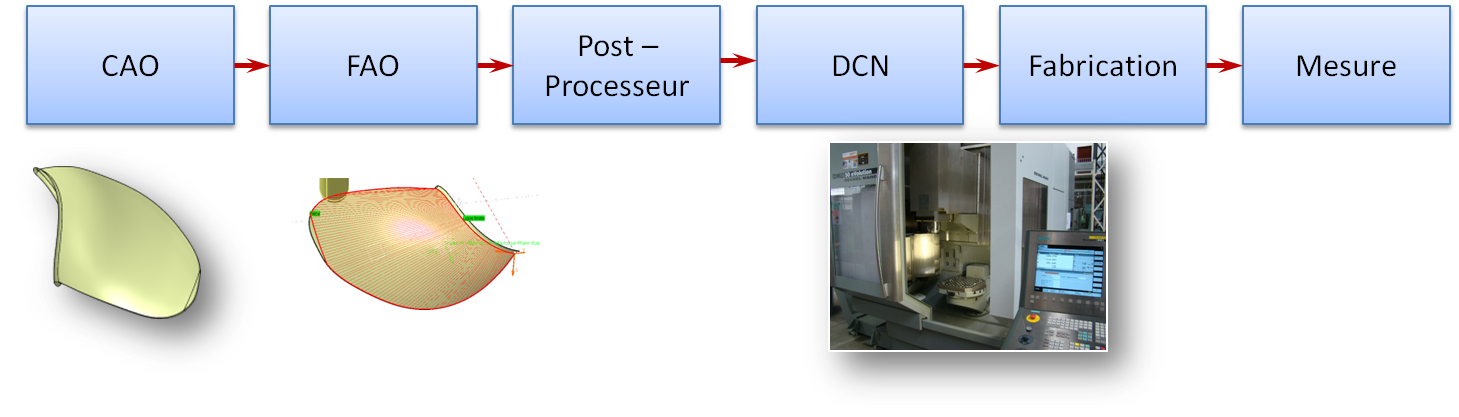
\includegraphics[width=.95\textwidth]{png/chaine_num}
\end{center}


\begin{center}
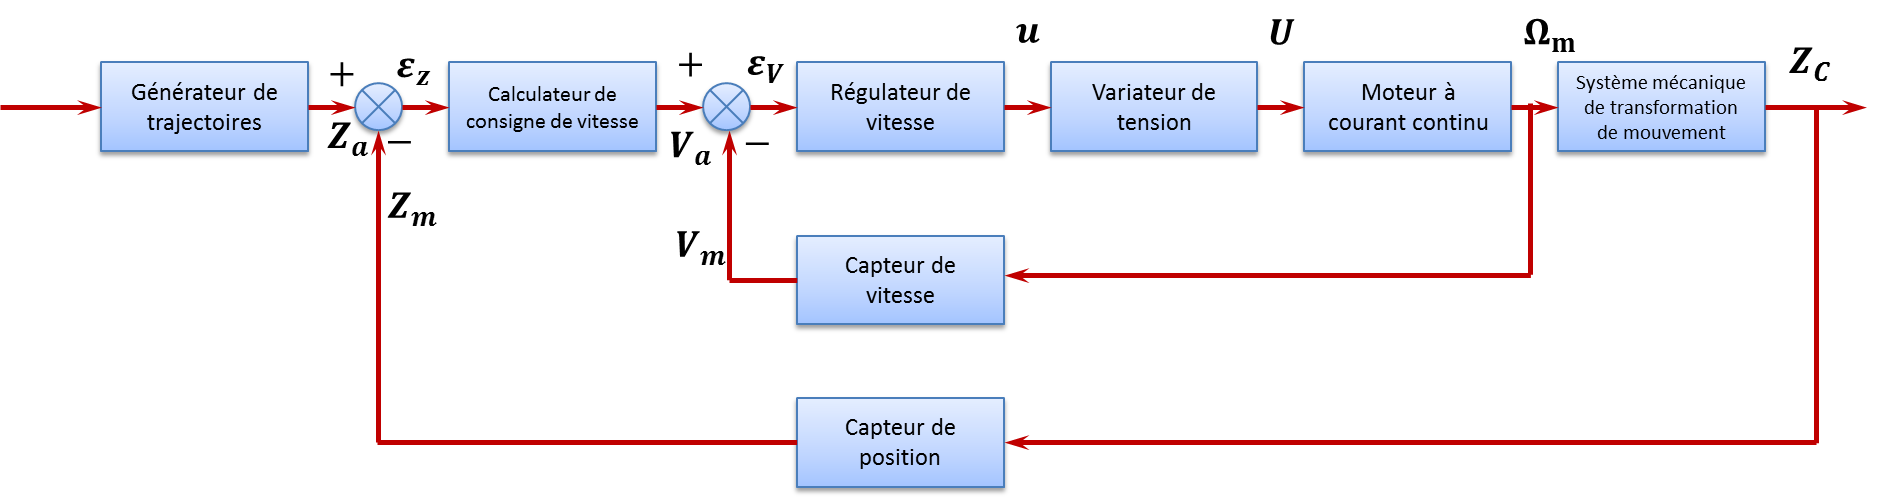
\includegraphics[width=.95\textwidth]{png/asservissement_cn}
\end{center}

\section{Typologie de pièces}
\paragraph*{Exemple de pièces réalisables en usinage 5 axes continus \cite{roeders}}

\begin{minipage}[c]{.24\linewidth}
\begin{center}
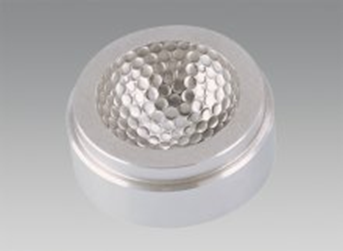
\includegraphics[width=.95\textwidth]{png/ex_1}

\textit{Matrice de balle de golf}
\end{center}
\end{minipage}\hfill
\begin{minipage}[c]{.24\linewidth}
\begin{center}
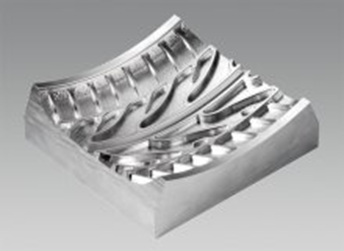
\includegraphics[width=.95\textwidth]{png/ex_2}

\textit{Matrice de pneu}
\end{center}
\end{minipage}\hfill
\begin{minipage}[c]{.24\linewidth}
\begin{center}
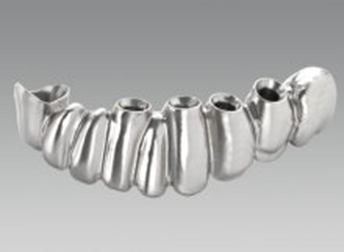
\includegraphics[width=.95\textwidth]{png/ex_3}

\textit{Prothèse de dents}
\end{center}
\end{minipage}\hfill
\begin{minipage}[c]{.24\linewidth}
\begin{center}
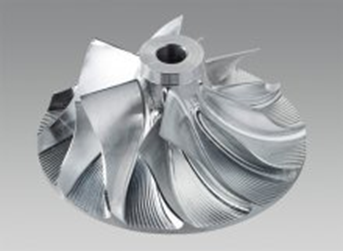
\includegraphics[width=.95\textwidth]{png/ex_4}

\textit{Rotor de turbomachine}
\end{center}
\end{minipage}

\section{Les porte-outils}

Sur une fraiseuse conventionnelle ou numérique, la liaison entre le porte-outil et la machine se fait par la broche. En fraisage à commande numérique, les machines possèdent généralement un magasin d'outil qui permet de les stocker. 

\begin{center}
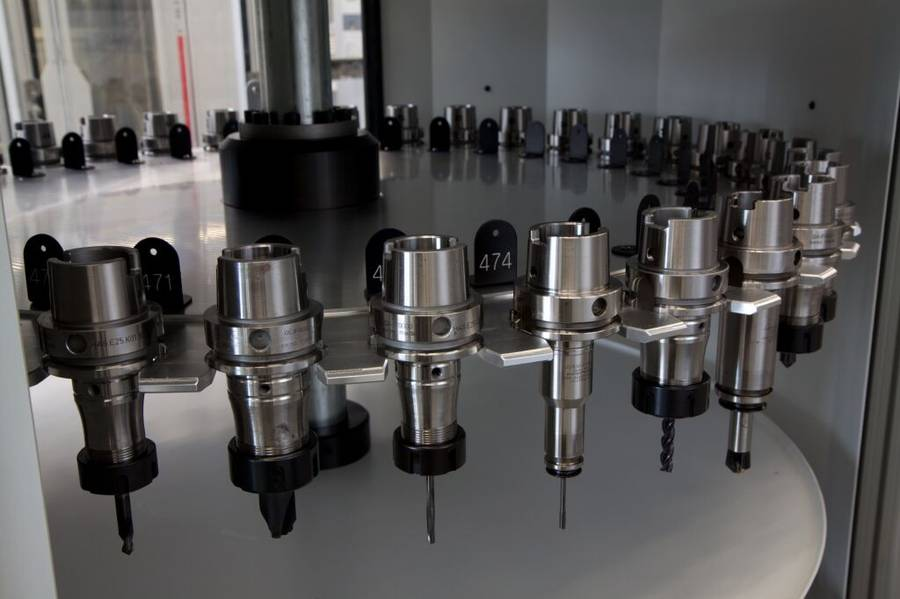
\includegraphics[height=5cm]{png/magasin_outil}

\textit{Magasin d'outil sur centre d'usinage}
\end{center}


En fraisage, le corps des outils est cylindriques. Deux solutions permettent de les maintenir en position dans le porte-outil. Un ajustement cylindre -- cylindre permet de les mettre en position. Le maintien en position est alors assuré par une vis appuyant sur un méplat. Le maintien en position peut aussi être assuré par un montage en pince. Le serrage de la pince permet le serrage de l'outil. 

La liaison entre la machine se fait par des attachements ISO qui ont une forme conique qui permet la mise en position du porte outil. L'entraînement est assuré par un lardon venant se loger dans une rainure. Enfin la mise en position de l'outil est assuré par une tirette positionnée en bout de porte-outil. 

Dans le cas des machines tournant à grande vitesse, on utilise des attachements HSK. La mise en position est aussi assurée par un cône. Le maintien en position est assuré par un dispositif venant à l'intérieur de l'attachement. Lorsque l'outil tourne, le serrage est alors accru grâce aux efforts centrifuges. 

\begin{minipage}[c]{.45\linewidth}
\begin{center}
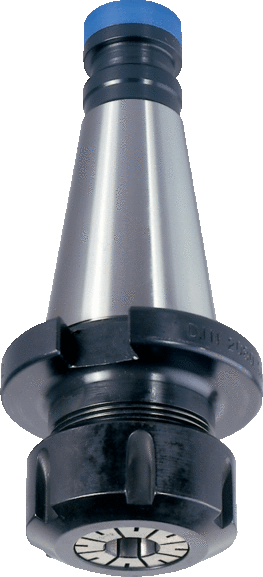
\includegraphics[height=5cm]{png/attachement_cone}

\textit{Attachement ISO}
\end{center}
\end{minipage}\hfill
\begin{minipage}[c]{.45\linewidth}
\begin{center}
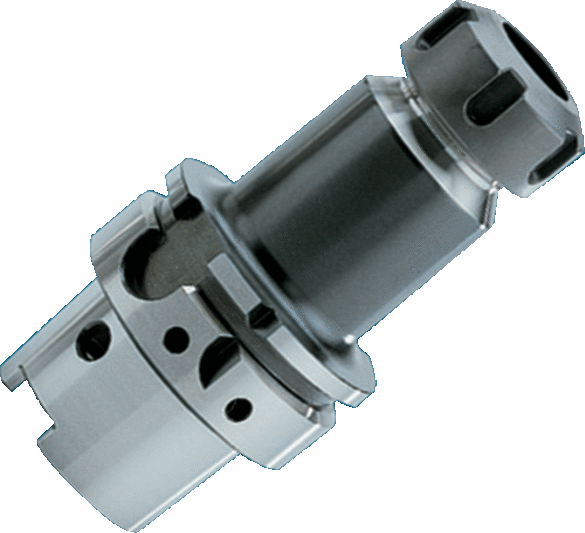
\includegraphics[height=5cm]{png/attachement_hsk}

\textit{Attachement HSK}
\end{center}
\end{minipage}

\section{Les outils}
\subsection{Géométrie des outils}

La géométrie des outils de fraisage dépend souvent de la géométrie de la forme à réaliser. Généralement, les outils de faible diamètre sont des outils monoblocs. Les outils de grands diamètres sont obtenus en utilisant un outil avec des plaquettes rapportées. 

Lorsqu'on parle des outils de fraisage, il faut distinguer le nombre de dents, et le nombre de coupes. Une fraise 5 dents 2 tailles possède par exemple 5 plaquettes. Chaque plaquette peut usiner avec deux arrêtes. 

\begin{minipage}[c]{.3\linewidth}
\begin{center}
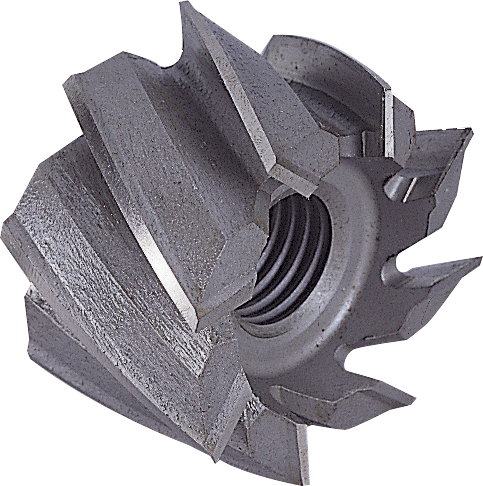
\includegraphics[width=.9\textwidth]{png/fr_2t}

\textit{Fraise 2 tailles -- 8 dents}
\end{center}
\end{minipage}\hfill
\begin{minipage}[c]{.3\linewidth}
\begin{center}
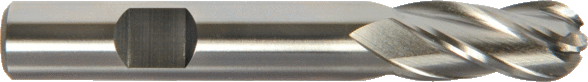
\includegraphics[width=.9\textwidth]{png/fr_hemisph}

\textit{Fraise hémisphérique -- 2 tailles -- 8 dents}
\end{center}
\end{minipage}\hfill
\begin{minipage}[c]{.3\linewidth}
\begin{center}
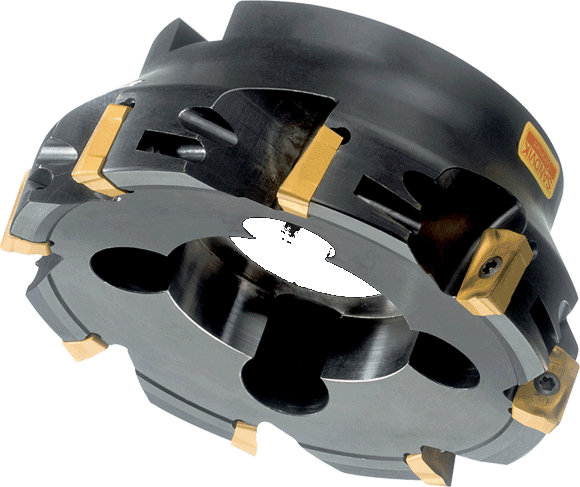
\includegraphics[width=.9\textwidth]{png/fr_surfacer}

\textit{Fraise à surfacer}
\end{center}
\end{minipage}



\subsection{Les opérations d'usinage}

\subsubsection{Surfaçage}
\begin{center}
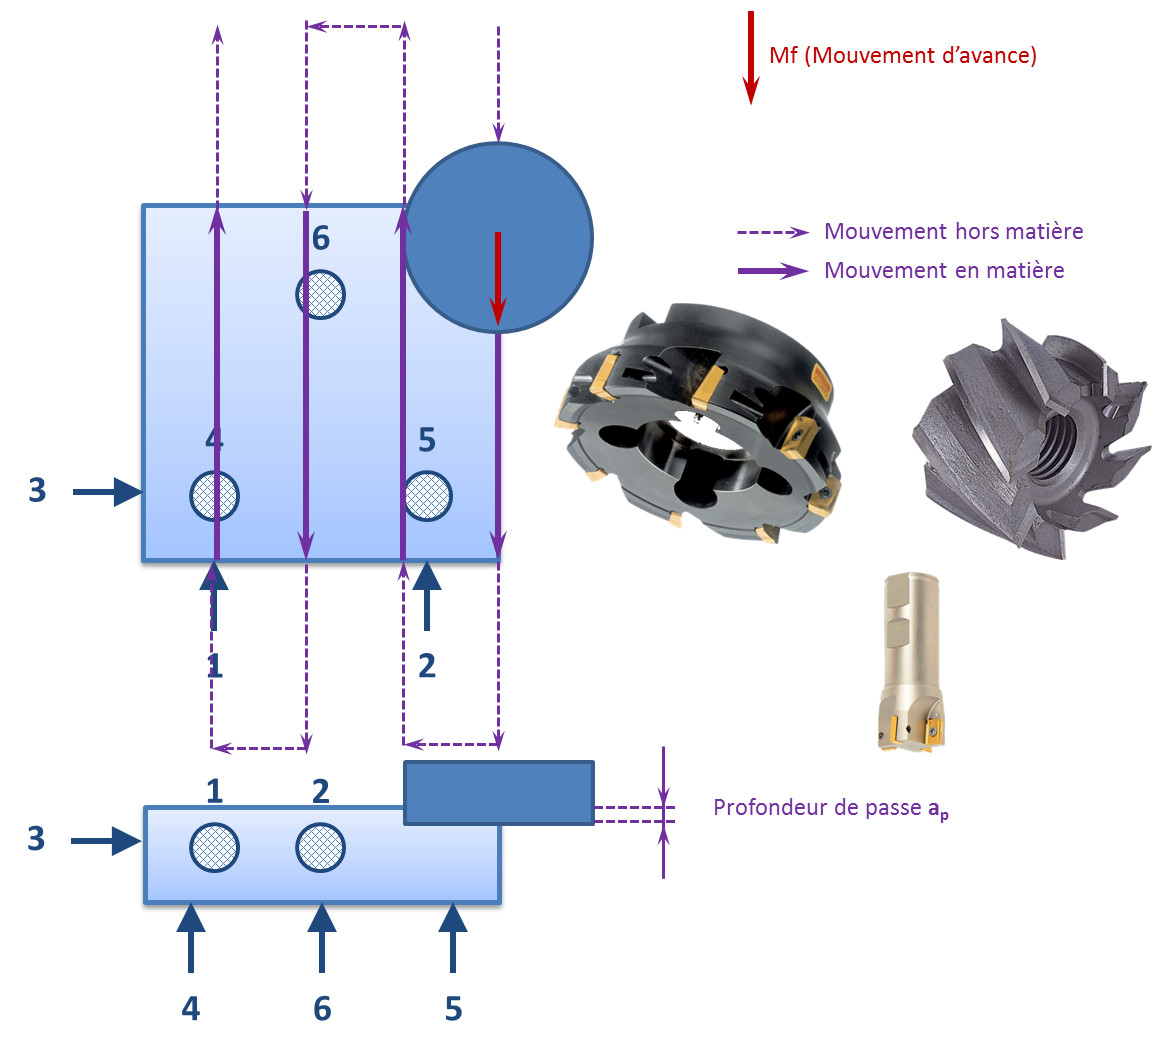
\includegraphics[width=.6\textwidth]{png/op_surfacage}
\end{center}
\subsubsection{Usinage sur le flanc}
\begin{center}
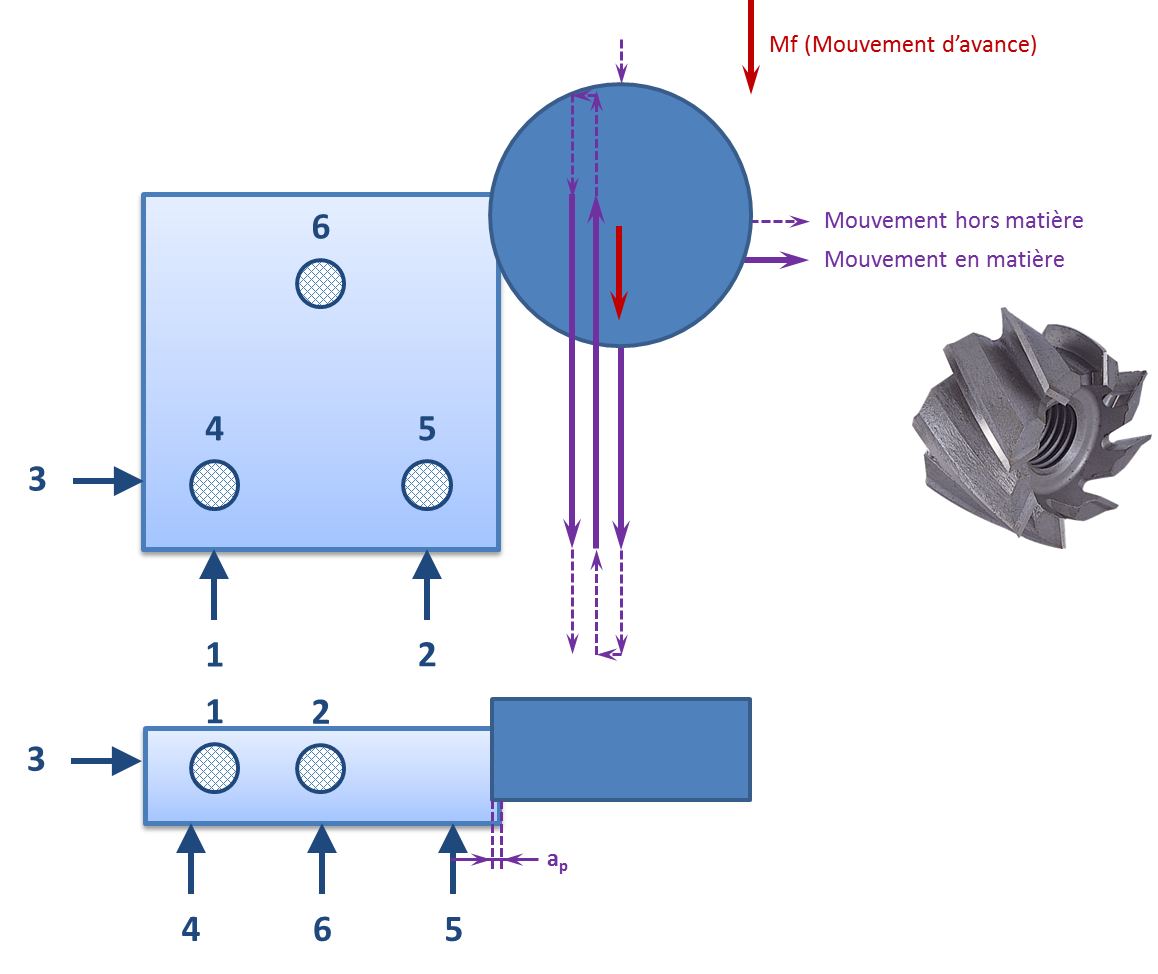
\includegraphics[width=.6\textwidth]{png/op_flanc}
\end{center}
\subsubsection{Rainurage}
\begin{center}
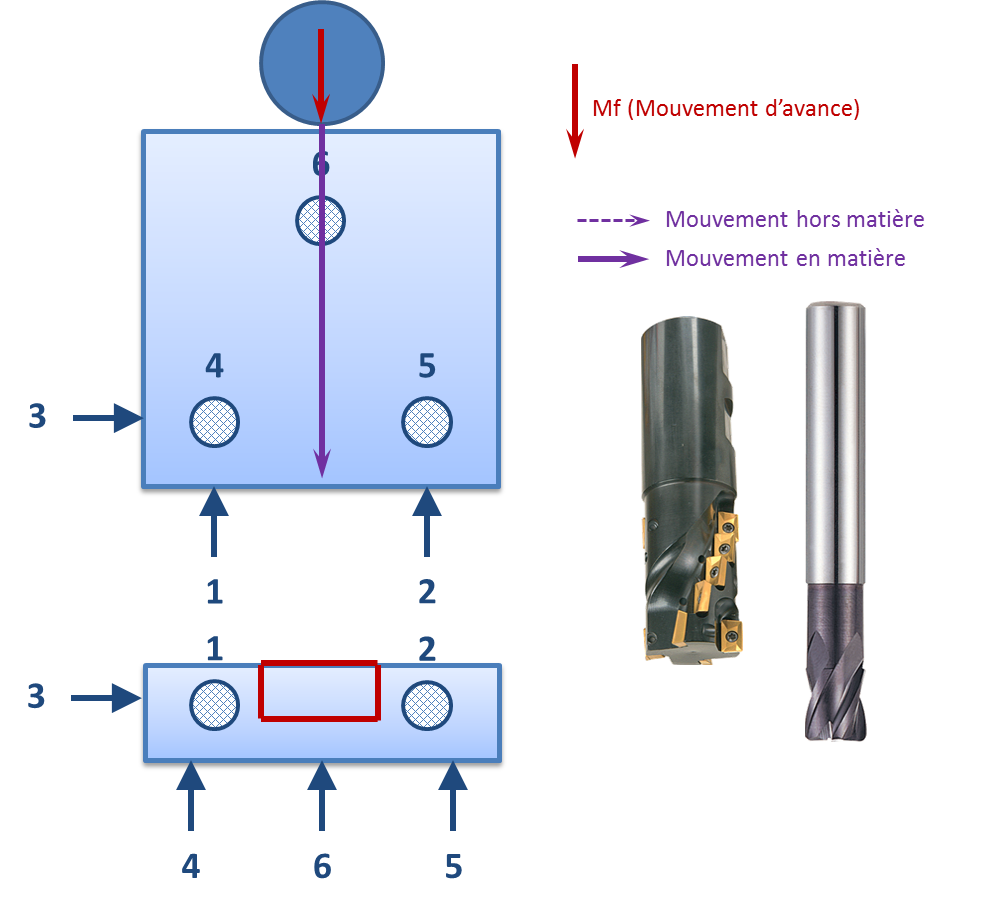
\includegraphics[width=.6\textwidth]{png/op_rainurer}
\end{center}
\subsubsection{Rainurage en T}
\begin{center}
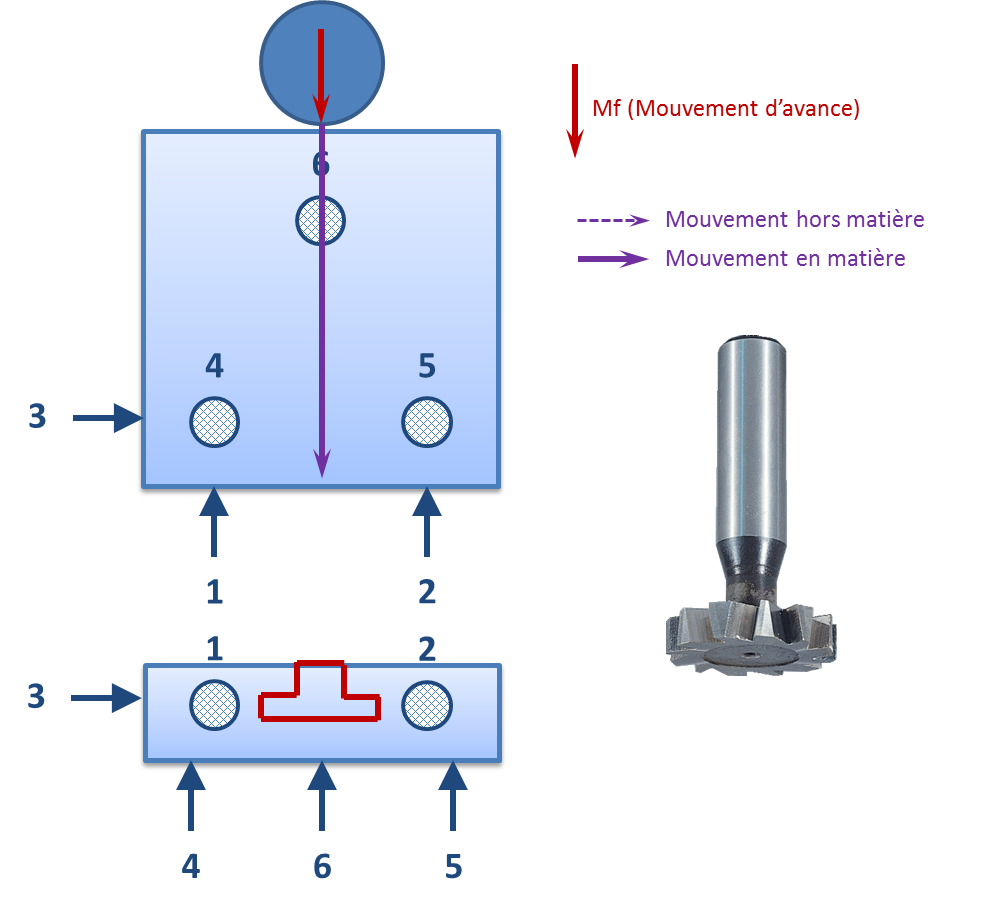
\includegraphics[width=.6\textwidth]{png/op_rainure_t}
\end{center}
\subsubsection{Usinage d'une queue d'aronde}
\begin{center}
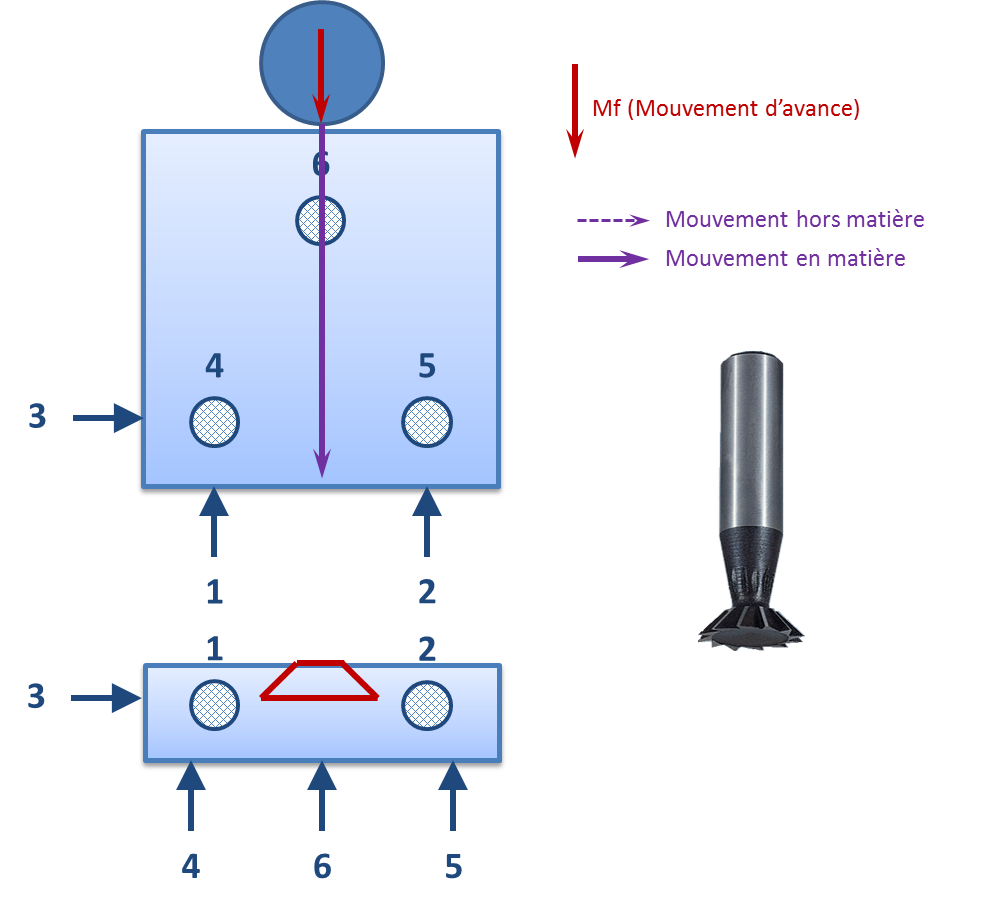
\includegraphics[width=.6\textwidth]{png/op_aronde}
\end{center}

\subsubsection{Usinage d'une forme quelconque}
\begin{center}
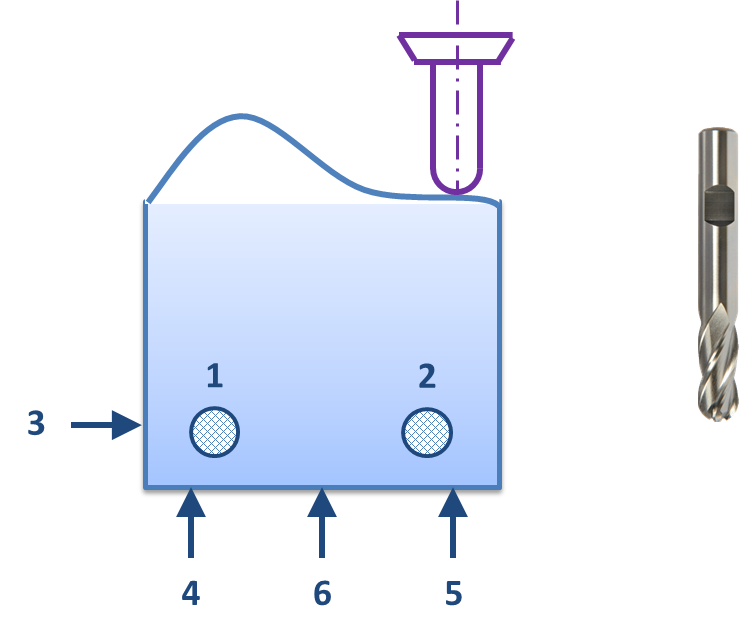
\includegraphics[width=.6\textwidth]{png/op_qq}
\end{center}

\subsubsection{Fraises 3 tailles à rainurer}

\begin{minipage}[c]{.2\linewidth}
\begin{center}
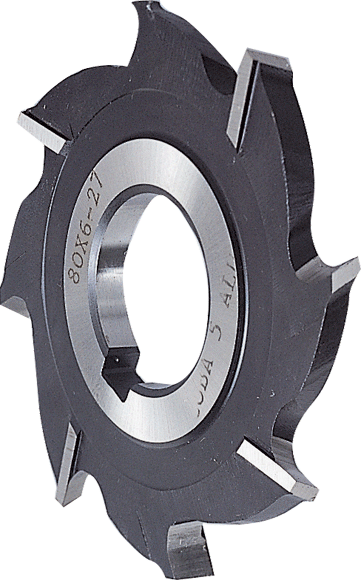
\includegraphics[height=4cm]{png/fr_3t}
\end{center}
\end{minipage} \hfill
\begin{minipage}[c]{.2\linewidth}
\begin{center}
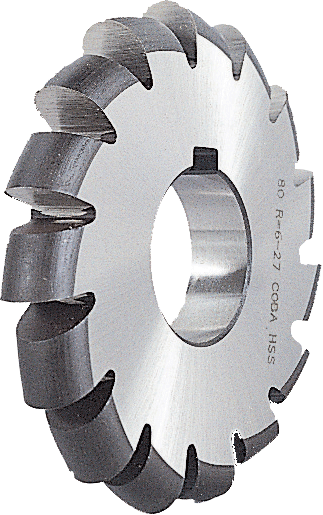
\includegraphics[height=4cm]{png/fr_3t_2}
\end{center}
\end{minipage} \hfill
\begin{minipage}[c]{.2\linewidth}
\begin{center}
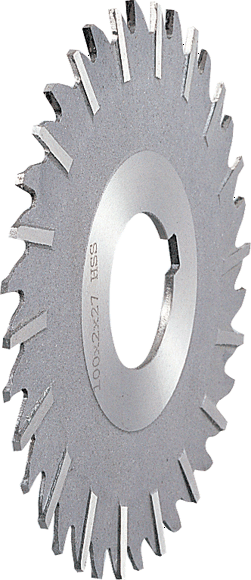
\includegraphics[height=4cm]{png/fr_disque}
\end{center}
\end{minipage} \hfill
\begin{minipage}[c]{.2\linewidth}
\begin{center}
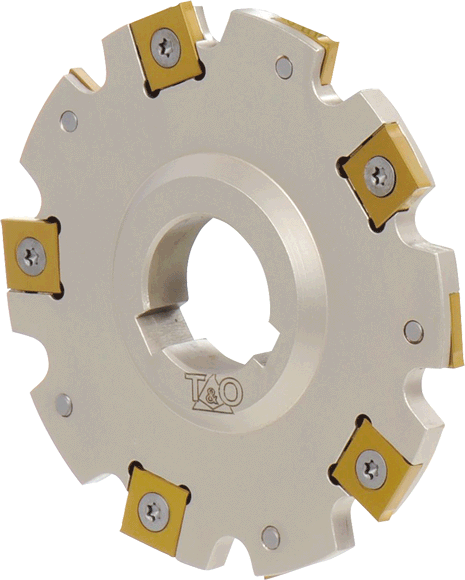
\includegraphics[height=4cm]{png/fr_disque_2}
\end{center}
\end{minipage} 

\subsubsection{Fraises à chanfreiner}

\begin{minipage}[c]{.45\linewidth}
\begin{center}
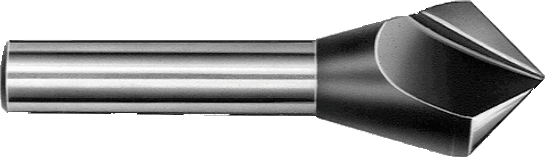
\includegraphics[width=.7\textwidth]{png/fr_chanfrein}
\end{center}
\end{minipage} \hfill
\begin{minipage}[c]{.45\linewidth}
\begin{center}
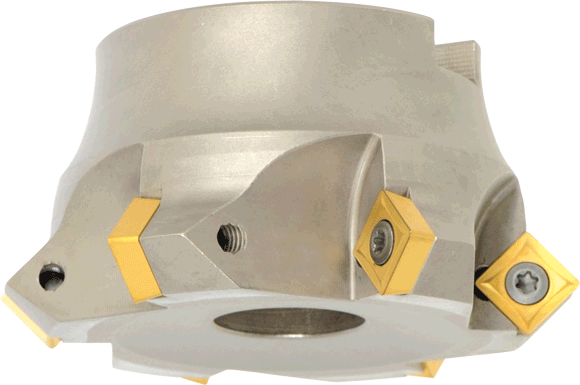
\includegraphics[width=.6\textwidth]{png/fr_chanfrein_2}
\end{center}
\end{minipage}

\section{Les portes pièces}
\subsection{Cahier des charges}

\begin{center}
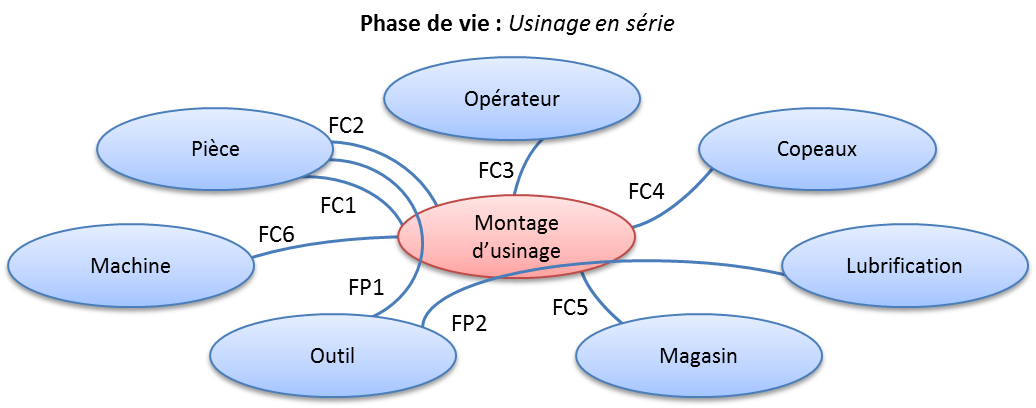
\includegraphics[width=.95\textwidth]{png/af1}
\end{center}

\begin{center}
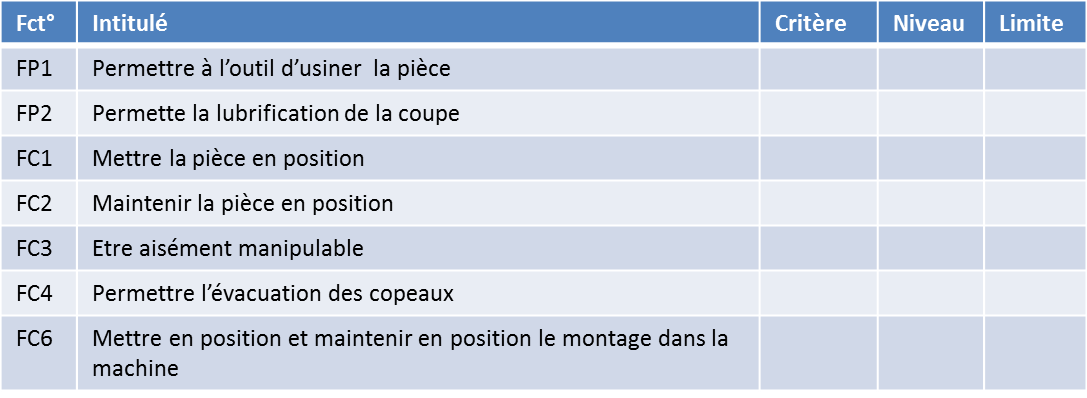
\includegraphics[width=.95\textwidth]{png/af2}
\end{center}


\subsection{Les portes pièces}
\subsubsection{Les portes pièces standards}
Les portes pièces désignent les étaux ou encore les plateaux magnétiques. Ils sont utilisés lors de la fabrication de pièces unitaires. Leur coût est relativement faible. 

\begin{minipage}[c]{.3\linewidth}
\begin{center}
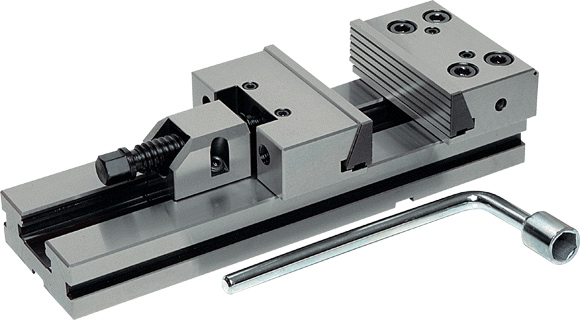
\includegraphics[width=.95\textwidth]{png/etau}

\textit{Étau}
\end{center}
\end{minipage} \hfill
\begin{minipage}[c]{.3\linewidth}
\begin{center}
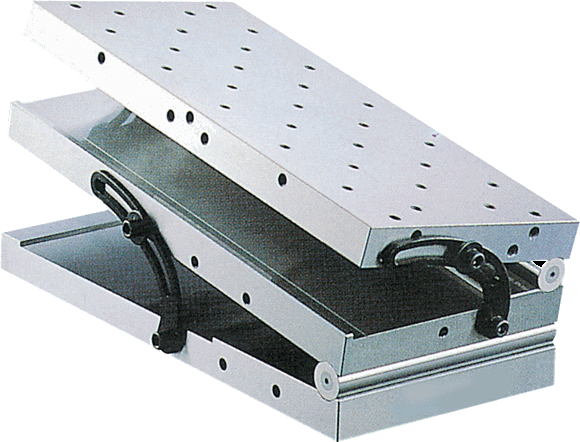
\includegraphics[width=.95\textwidth]{png/sinus}

\textit{Table sinus}
\end{center}
\end{minipage}\hfill
\begin{minipage}[c]{.3\linewidth}
\begin{center}
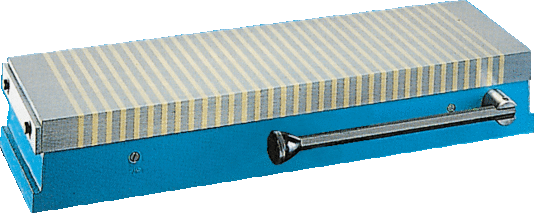
\includegraphics[width=.95\textwidth]{png/table_magnetique}

\textit{Table magnétique}
\end{center}
\end{minipage}


\subsubsection{Les portes pièces modulaires}
Les portes pièces modulaires sont utilisés pour la fabrication de pièces en moyenne série. Ils sont composés de modules standards qui permettent de mettre en position la pièce et de la maintenir en position. Ces portes pièces nécessitent un investissement dans l'achat des modules ainsi qu'un coût d'étude avant d'industrialiser la pièce. 

\begin{minipage}[c]{.3\linewidth}
\begin{center}
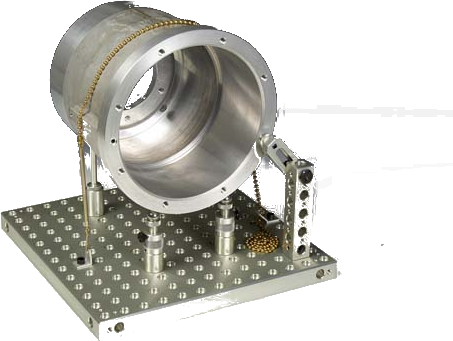
\includegraphics[width=.95\textwidth]{png/modulaire_1}
\end{center}
\end{minipage} \hfill
\begin{minipage}[c]{.3\linewidth}
\begin{center}
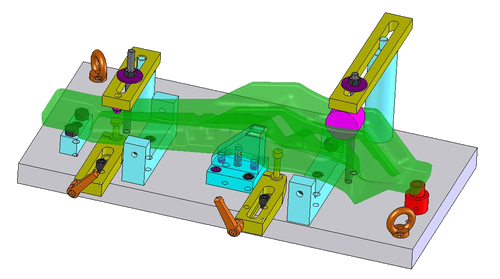
\includegraphics[width=.95\textwidth]{png/modulaire_2}
\end{center}
\end{minipage}\hfill
\begin{minipage}[c]{.3\linewidth}
\begin{center}
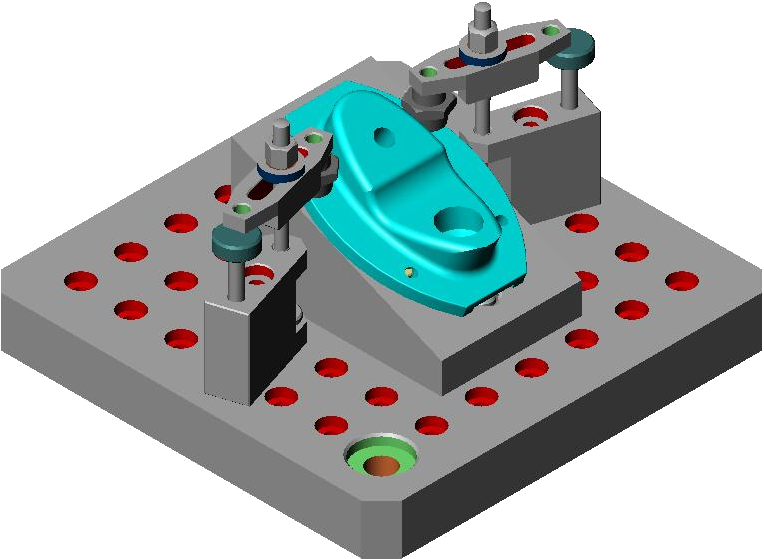
\includegraphics[width=.95\textwidth]{png/modulaire_3}
\end{center}
\end{minipage}


\subsubsection{Les portes pièces spécifiques}

Ils sont réservés à l'usinage des pièces en grande série. Ces portes pièces nécessitent eux-mêmes un coût de conception et de fabrication.



\subsection{Mise en position isostatique des pièces}
Sur un contrat de phase (voir partie suivante), il est nécessaire d'indiquer comment sera positionnée la pièce dans la machine. Cette mise en position est indépendante du porte-pièce. Il ne s'agit que d'une représentation symbolique.

La mise en position de la pièce permet de mettre en évidence comment sera réalisée la liaison encastrement entre la pièce et le porte-pièce. Afin de réaliser une liaison encastrement, il faut bloquer 6 degrés de liberté qui seront représentés par des flèches numérotées. 

Le choix de la mise en position dépend :
\begin{itemize}
\item de la cotation de la pièce;
\item de l'étendue des surfaces;
\item de l'accessibilité des surfaces.
\end{itemize}

\begin{center}
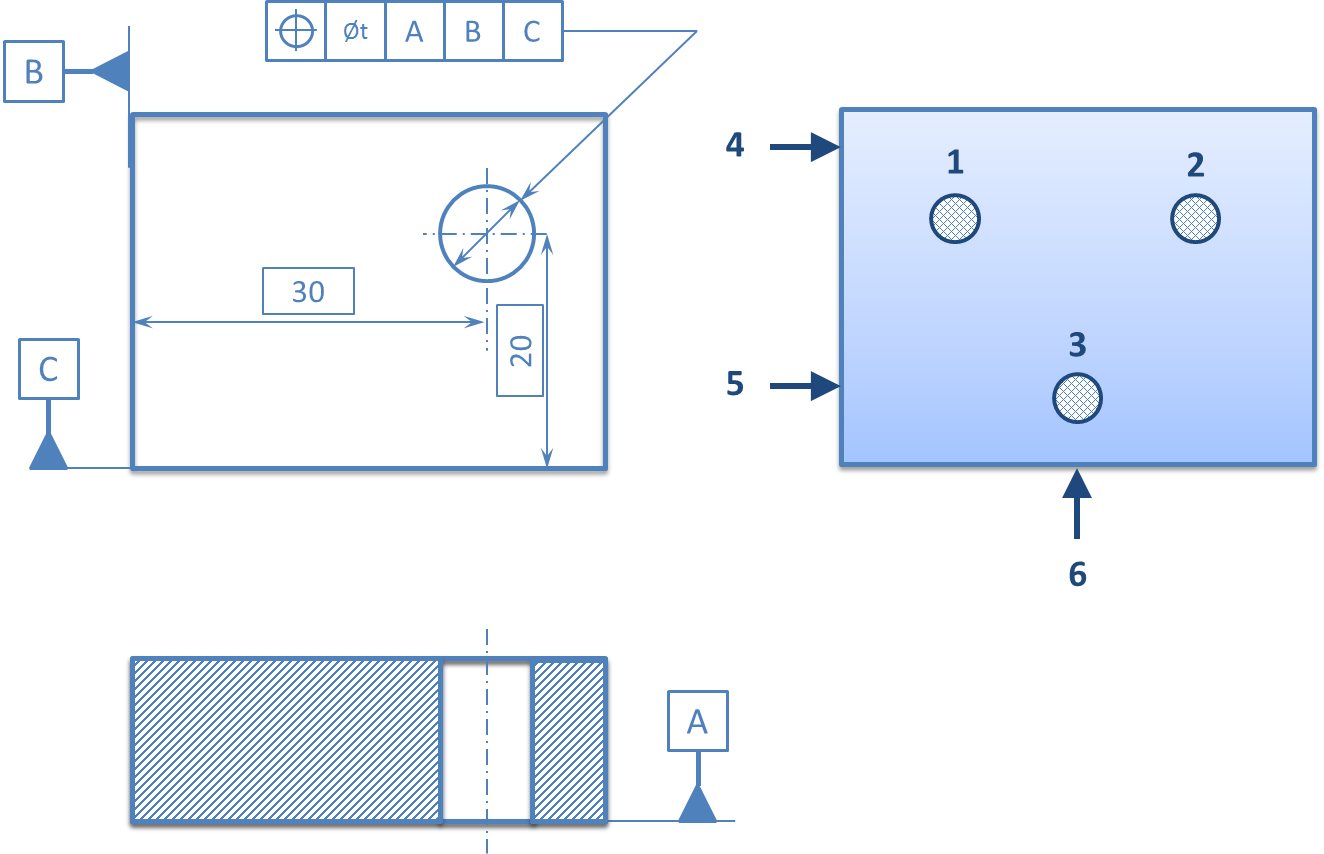
\includegraphics[width=.8\textwidth]{png/MIP_1}
\end{center}


\begin{center}
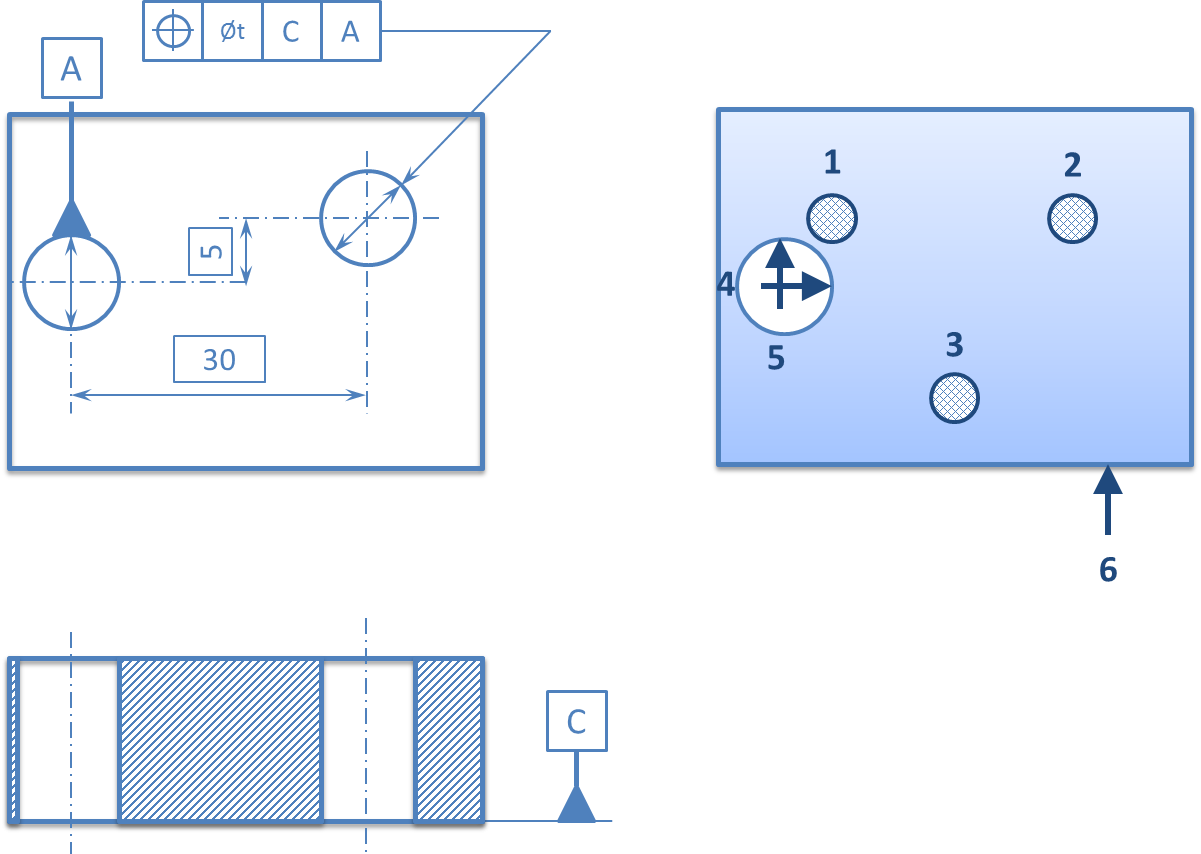
\includegraphics[width=.8\textwidth]{png/MIP_2}
\end{center}








\section{Contrat de phase}
\begin{defi}
Un contrat de phase est un document comportant toutes les opérations présentes dans une phase. Une phase correspond à un posage (une mise en position) unique de la pièce.
\end{defi}


\subsection{Ordonnancement des phases}


%
%Pour usiner la pièce, deux solutions semblent possibles initialement. Commencer par la partie "gauche" ou par la partie "droite". 
 
\begin{methode}
Pour choisir comment ordonnancer les phases, il est nécessaire de s'appuyer sur les spécifications.  Dans la mesure du possible on commence par usiner \textbf{les surfaces de références} des spécifications.

Les surfaces de références devront alors être utilisées pour réaliser la \textbf{mise en position de la pièce} lors de l'usinage des surfaces spécifiées.
\end{methode}


\subsection{Ordonnancement des opérations}
Il n'existe pas forcément de méthode rigoureuse pour ordonnancer les opérations. Le bon sens est souvent de rigueur. 

Lorsqu'il faut enlever une grande quantité de matière on commencera par réaliser une ébauche pour enlever une grande quantité de matière et avec le plus grand débit possible pour être productif. Une finition permettra alors d'obtenir la dimension finale et la qualité de surface souhaitée.
\subsection{Exemple}

On désire réaliser la pièce suivante à partir d'un brut parallélépipédique. Proposer un ordonnancement des phases et des opérations.
\begin{center}
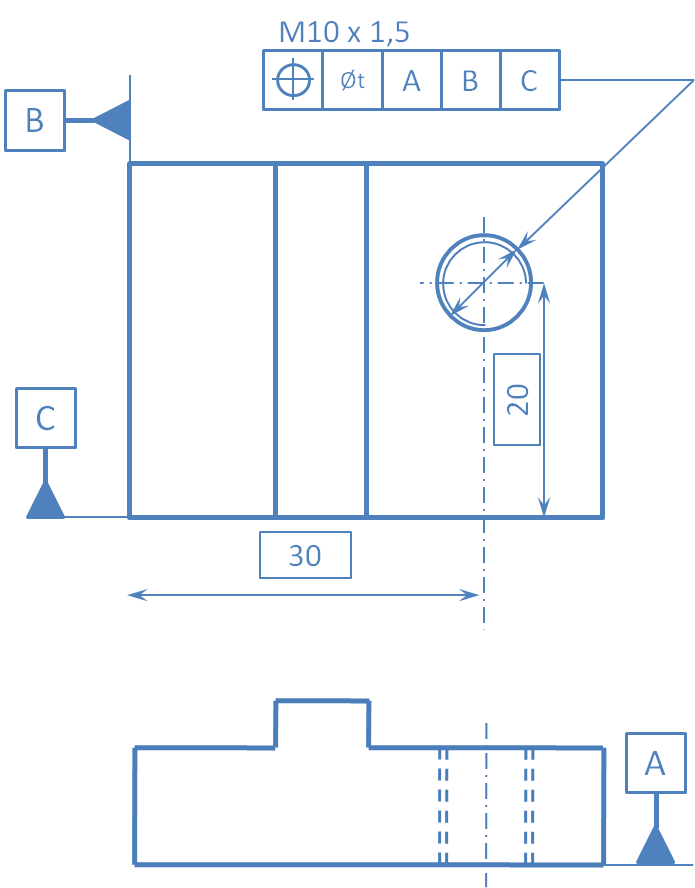
\includegraphics[width=.5\textwidth]{png/exemple_gamme}


\end{center}

\subsection{Conditions de coupe}

\begin{defi}
\textbf{Conditions de coupe}

En fraisage, déterminer les conditions de coupe revient à déterminer : 
\begin{itemize}
\item la vitesse de coupe;
\item la vitesse d'avance; 
\item la profondeur de passe et l'engagement de la fraise.
\end{itemize}
\end{defi}

\begin{defi}
\textbf{Vitesse de coupe}

La vitesse de coupe correspond à la vitesse de l'arrête de coupe par rapport à la pièce. 

Elle est donnée par le couple outil matière, c'est-à-dire par la combinaison du matériau de l'outil et de la pièce. On la note $V_c$ et s'exprime en $m/min$. La vitesse de coupe permet de déterminer la vitesse de rotation de la broche. On la note $N$ en $tr/min$. 

On montre aisément que 
$$
N= \dfrac{1000\cdot V_c}{\pi D}
$$

Dans cette formule, $N$ est exprimé en $tr/min$, $V_c$ en $m/min$ et $D$ en $mm$.
\end{defi}

%% Vitesse de coupe

\begin{defi}
\textbf{Vitesse d'avance}

La vitesse d'avance correspond à la vitesse d'avance de l'outil sur la trajectoire d'usinage. On note $V_f$ la vitesse d'avance en $mm/min$. 

En fonction du matériau à usiner, le constructeur d'outil préconise une vitesse d'avance par tour et par dent. On la note $f_z$ en $mm/tr/dent$ 

La vitesse d'avance $V_f$ en $mm/min$ est donnée par $V_f = N\cdot f_z \cdot Z$ avec $Z$ le nombre de dents de la fraise. 
\end{defi}

%% Détermination de la vitesse d'avance, diagramme brise copeau.

\begin{defi}
\textbf{Profondeur de passe et engagement}

Le choix de la profondeur de passe dépend de plusieurs paramètres. On la note $a$ en $mm$. 

Un choix judicieux de la profondeur de passe peut permettre d'augmenter la productivité. 

Cependant une grande profondeur de passe demande de plus grand efforts de coupe. Il faut alors que les efforts générés soient compatibles avec la puissance de la machine.

L'engagement correspond à la proportion de la fraise qui va être engagée lors de l'usinage.
	
\end{defi}

\begin{exemple}
\begin{center}
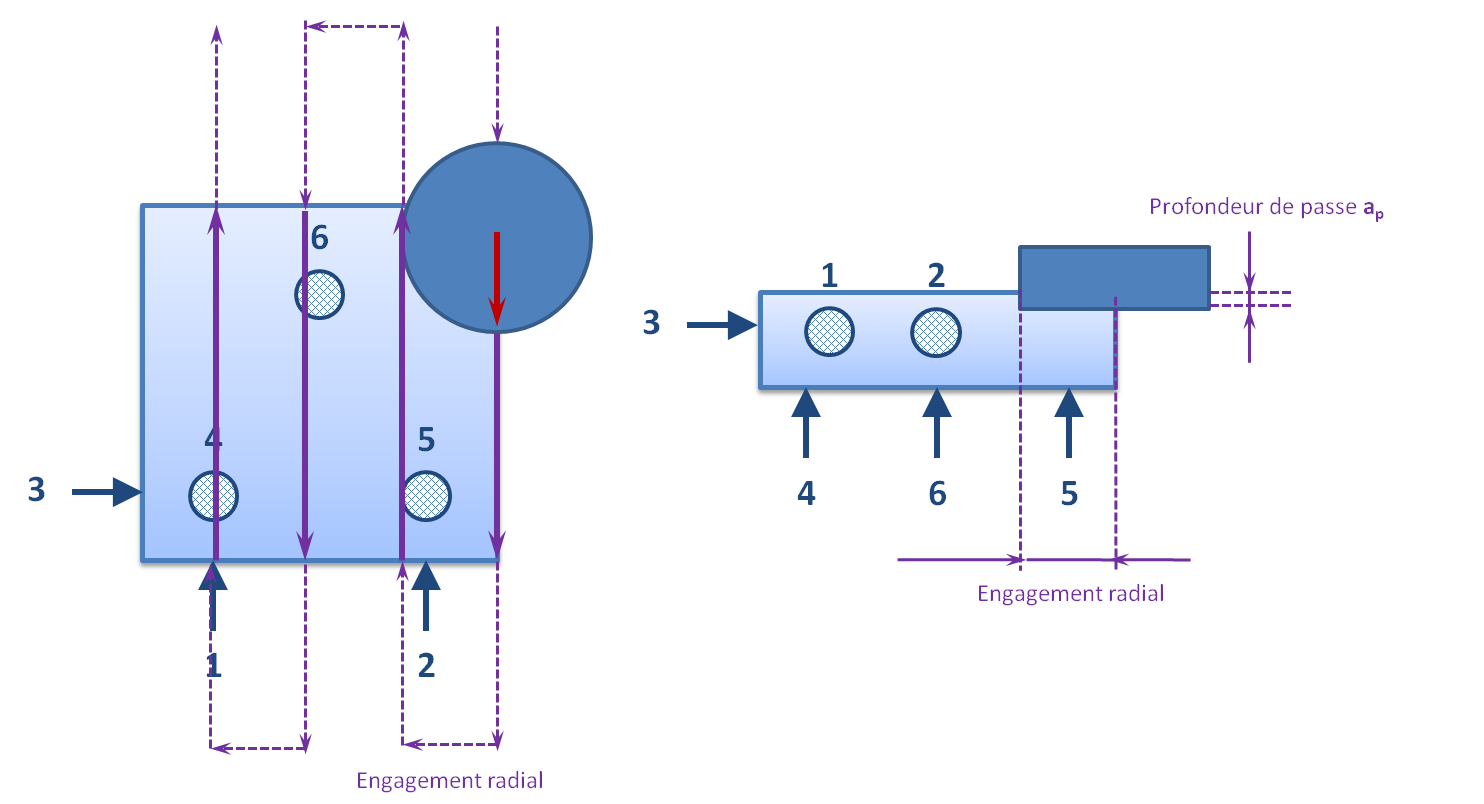
\includegraphics[width=.8\textwidth]{png/engagement_radial}
\end{center}
\end{exemple}

\begin{thebibliography}{2}
\bibitem{dent}{\url{http://www.zeta-dental.fr/images/upload/Image/16519-1.jpg}}
\bibitem{conventionnel}{\url{http://www.hellopro.fr/images/produit-2/7/9/1/fraiseuse-conventionnelle-2654197.jpg}}
\bibitem{5axes}{\url{http://fr.dmg.com/fr,milling,dmu-60-evo-linear?opendocument}}
\bibitem{fraises}{\url{http://www.walter-tools.com/}}
\bibitem{otelo}{\url{www.otelo.fr/}}
\bibitem{roeders}{\url{http://www.roeders.de/}}
\end{thebibliography}

\end{document}